\documentclass[12pt, letterpaper]{article}
\usepackage{graphicx} % Required for inserting images
\usepackage{hyperref}
\usepackage{listings}
\usepackage{amssymb}
\usepackage{amsmath}
\usepackage[english]{babel}
\usepackage{nicefrac, xfrac}
\usepackage{mathtools}
\usepackage[table,xcdraw]{xcolor}
\definecolor{light-gray}{gray}{0.95}
\definecolor{sap}{RGB}{130, 36, 51}
\definecolor{lg}{RGB}{102, 161, 95}
\definecolor{g}{RGB}{60, 50, 50}
\usepackage[paper=a4paper,left=20mm,right=20mm,bottom=25mm,top=25mm]{geometry}
\newcommand{\code}[1]{\colorbox{light-gray}{\texttt{#1}}}
\newcommand{\shelll}[1]{\colorbox{black}{\textcolor{white}{\texttt{#1}}}}
\newcommand{\shell}[1]{\colorbox{black}{\textcolor{white}{\texttt{casufrost@debian:$\sim$\$ #1}}}}
\newcommand{\codee}[1]{\colorbox{white}{\texttt{#1}}}
\newcommand{\acc}{\\\hphantom{}\\}
\newcommand{\dete}{{\rightarrow}}
\newcommand{\fdot}{{\(\bullet\) }}
\newcommand{\comm}[1]{\color{lg}\textit{\hphantom{spaz}// \text{#1}}\color{black}}
\newcommand{\textg}[1]{\color{g}{\textbf{#1}}\color{black}}
\newcommand{\boxedMath}[1]{\begin{tabular}{|c|}\hline \texttt{#1} \\ \hline\end{tabular} :}
\title{Reti di Elaboratori}
\author{Marco Casu}
\date{\vspace{-5ex}}
\begin{document}



\maketitle
\begin{figure}[h]
    \centering{
        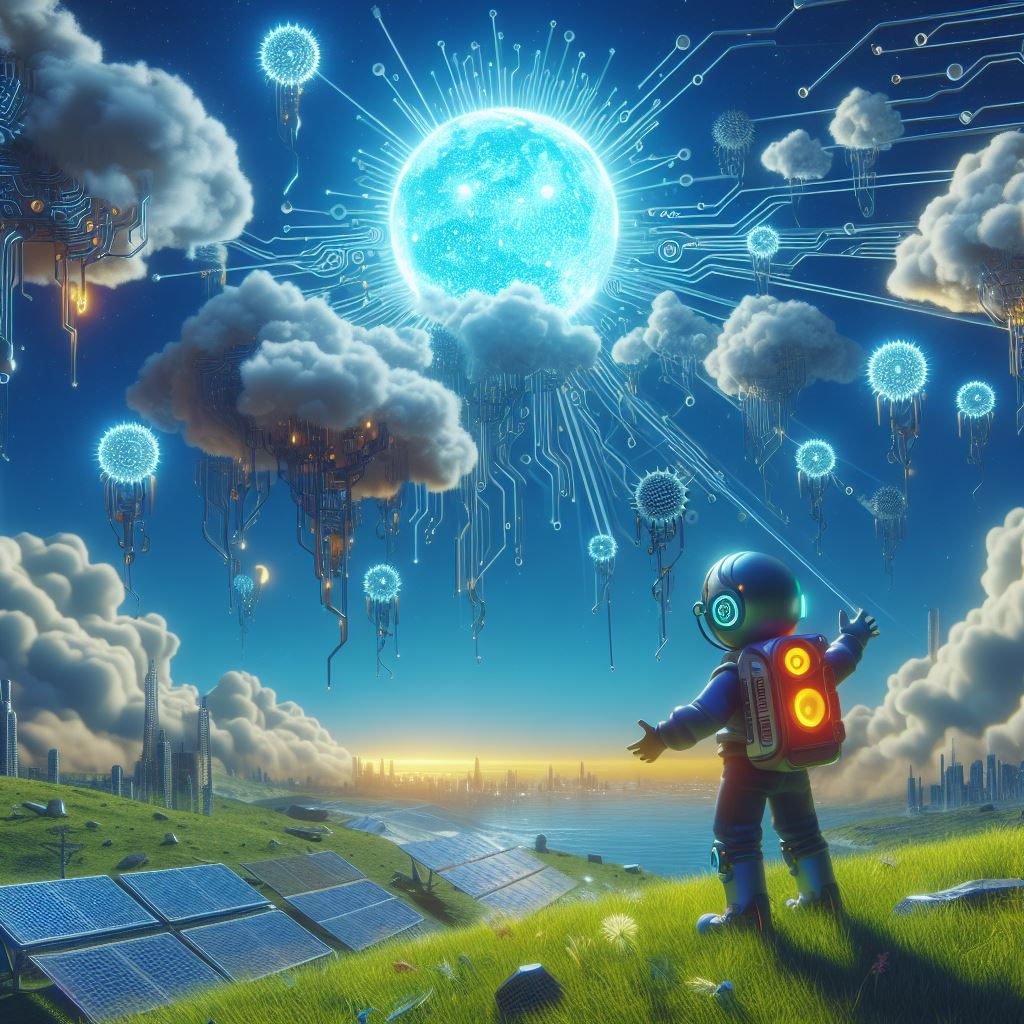
\includegraphics[width=1\textwidth ]{images/cop.jpg}
    }
\end{figure}
\newpage
\tableofcontents
\newpage
\section{Reti di Calcolatori e Internet}
Cos'è una richiesta di rete? E soprattutto quali sono i passaggi ed il procedimento scaturito a seguito di una richiesta? Questo corso
si concentrerà sull'aspetto del \textit{networking}, ossia, su come avviene la comunicazione tramite più elaboratori.\acc
Una \textit{connessione} è una comunicazione aperta in cui sono coinvolte entrambe le parti in attesa di ricevere ed inviare
messaggi, tramite l'apertura di un \textit{socket} (si approfondirà in seguito). Il problema di una comunicazione di questo tipo,
è il bisogno di avere la certezza che i messaggi inviati da una parte siano ricevuti correttamente dall'altra, senza il rischio di
comunicare "a vuoto", per questo sono definiti degli appositi protocolli.\acc
\textbf{Host} : Un dispositivo connesso alla rete in modo periferico, non funge da esclusivo tramite per la comunicazione,
ed è un sistema "periferico", esegue delle \textit{app} che forniscono servizi sulla rete.\acc
\textbf{Switch} : Gli switch sono i dispositivi capaci di "instradare" i \textit{pacchetti}.\acc
\textbf{Rete} : Una collezione di dispositivi host/switch e collegamenti gestiti da un unico ente/organizzazione.\begin{center}
    \includegraphics[width=1\textwidth ]{images/reteDef.eps}
\end{center}
Quella che noi chiamiamo \textbf{internet}, è una "\textit{rete di reti}", ossia l'insieme interconnesso di tutte le reti
pubbliche, che si stabilisce e necessita di protocolli su tutti i livelli : \begin{itemize}
    \item Livello di applicazione
    \item Livello di trasporto
    \item Livello network
    \item Livello di collegamento
\end{itemize}
Lo scopo di internet è quello di essere un infrastruttura che fornisce i servizi alle applicazioni distribuite, è
un interfaccia di programmazione e fornisce un servizio di \textit{trasporto dei dati}.\acc
Un \textbf{protocollo di rete}, stabilisce delle regole riguardanti lo scambio di messaggi, con le relative "azioni" specifiche
da intraprendere per la ricezione di messaggi ed eventi, definiscono il \textit{formato} e \textit{l'ordine} dei messaggi
da inviare fra le entità di rete, e le azioni intraprese sulla ricezione e trasmissione dei messaggi.
\subsection{Struttura di Internet e Link}
Una rete è quindi un insieme di nodi collegati tramite dei \textit{link}, composta da dispositivi di interconnessione, che
si scambiano informazioni, usualmente utilizziamo il termine \textit{host} per i dispositivi che usufruiscono di un servizio,
e \textit{server} per i dispositivi che lo erogano.\acc
I dispositivi di interconnessione, ricevono un segnale, lo modificano e lo ritrasmettono, sono i \textit{router} (collegano una
rete ad altre reti) e gli  \textit{switch} (collegano più dispositivi ad una rete locale). I collegamenti, o link, possono
essere cablati (rame o fibra ottica) oppure wireless, senza cavi (onde elettromagnetiche).\acc
Le reti locali come quelle casalinghe o aziendali, si collegano ad una rete regionale ISP (internet service provider) di router interconnessi detta
\textit{core} o \textit{backbone}, che a sua volta si collega ad una simile struttura ma a livello nazionale o globale.\acc
\subsubsection{Reti Cablate e Wireless}
Nell'accesso via cavo, c'è un terminale comune per più abitazioni detto \textbf{CMTS}, ossia \textit{Cable Modem Termination System},
che viene poi diramato nelle diverse abitazioni, i dati dalla rete ed i segnali per la televisione sono trasmessi sul medesimo
cavo ma a frequenze differenti. Il CMTS è direttamente collegato ad un ISP. In questo modello diverse case condividono la rete di
accesso.\begin{center}
    \includegraphics[width=1.1\textwidth ]{images/cableHeadend.eps}
\end{center}
La \textbf{DSL} diversamente, utilizza la linea telefonica esistente, collegandosi alla DSLAM, i dati sulla linea
DSL vanno su internet, la voce su DSL va sulla linea telefonica. \acc
In una rete \textit{domestica}  c'è un \textit{modem}
(si occupa di ricevere il segnale analogico e di  \textit{modularlo} in segnale digitale)
connesso ad un CMTS, collegato via cavo ad
un router, collegato direttamente tramite \textit{ethernet} agli host, oppure collegato ad un \textit{access point WI-FI} che
permette la connessione senza fili, questi utlimi tre molto spesso sono combinati in un unico device.\acc
La connessione senza fili, o wireless connette i sistemi terminali (host) al router, tramite il già citato
access point, esistono reti locali senza fili (WLAN), che hanno una copertura di circa 30 metri, e reti di accesso
cellulare \textit{wide area}, utilizzate dai dispositivi mobili e fornite da un operatore di rete cellulare, ed hanno una
copertura più ampia, nell'ordine dei kilometri.\acc
Le reti aziendali, come quelle delle università sono di una scala diversa rispetto quelle domestiche, prevedono molti più
dispositivi, ed un mix di varie tecnologie di collegamento, cablate o wireless, tramite svariati switch e router.
\subsubsection{Comunicazione e Classificazione delle Reti}
Un host comunica tramite l'invio e la ricezioni di messaggi da un applicazione sottoforma di \textit{pacchetti} di dati, ossia
messaggi suddivisi in blocchi più piccoli, di lunghezza $L$ bit. L'host trasmettono i pacchetti nella rete
ad una \textit{velocità di trasmissione} di $R$ $\nicefrac{bit}{sec}$. Il \textit{ritardo} di trasmissione del pacchetto è
il tempo necessario per trasmettere il pacchetto ($L$ bit) nel collegamento, ed equivale a $\dfrac{L}{R}$ secondi.\acc
Il segnale si propaga fra trasmettitore e ricevitore, tramite \textit{supporti guidati}, ossia i mezzi solidi (cavi), oppure
\textit{non guidati}, propagandosi liberamente nell'aria (onde elettromagnetiche).\begin{itemize}
    \item Il \textbf{cavo coassiale} è provvisto di due conduttori di rame concentrici, è bidirezionale, supporta più canali
          date diverse frequenze, ed è resistente alle interferenze.
    \item La \textbf{fibra ottica} ha soppiantato il cavo coassiale, è una fibra di vetro che trasporta impulsi luminosi, dove ciascun
          impulso rappresenta un bit, la luce rimbalza nel cavo muovendosi ad alta velocità, è necessario però considerare dei
          ripetitori (anche se molto distanziati), dato che la luce rimbalzando potrebbe tendere a disperdersi causando una perdita
          di informazioni.
    \item La rete \textbf{wireless} non ha un supporto guidato, il segnale è propagato nell'aria, è quindi \textit{broadcast},
          chiunque può ricevere il segnale. Tale metodo di comunicazione è \textit{half-duplex}, ossia, la comunicazione avviene da un
          mittente ad un destinatario, e non è possibile comunicare fra due enti contemporaneamente, è soggetta ad effetti dovuti all'ambiente
          di propagazione, come interferenze, riflessione e ostruzione da parte di oggetti fisici.
\end{itemize}
Esiste una scala di classificazione delle reti :\begin{center}
    \begin{tabular}{|
            >{\columncolor[HTML]{EFEFEF}}c |
            >{\columncolor[HTML]{FFFFFF}}c |c|
            >{\columncolor[HTML]{FFFFFF}}c |}
        \hline
        \cellcolor[HTML]{9AFF99}{\color[HTML]{000000} Scala} & \cellcolor[HTML]{9AFF99}Tipo & \cellcolor[HTML]{9AFF99}Nome completo & \cellcolor[HTML]{9AFF99}Esempio \\ \hline
        Distanza ravvicinata                                 & PAN                          & Personal Area Network                 & Bluetooth                       \\ \hline
        Edificio                                             & LAN                          & Local Area Network                    & WiFi, Ethernet                  \\ \hline
        Città                                                & MAN                          & Metropolitan Area Network             & Cablata, DSL                    \\ \hline
        Paese                                                & WAN                          & Wide Area Network                     & Grandi ISP                      \\ \hline
        Pianeta                                              & Internet                     & La rete di tutte le reti              & L'Internet                      \\ \hline
    \end{tabular}
\end{center}
La \textbf{LAN} è la rete locale, come una rete domestica, è una rete privata ed ogni terminale connesso ad essa è identificato
da un indirizzo distinto dagli altri, può essere a \textit{cavo condiviso} oppure a \textit{commutazione} con uno switch.\begin{center}
    \includegraphics[width=1\textwidth ]{images/cavocondiviso.eps}
\end{center}
In tale modello di cavo condiviso il pacchetto inviato ad un dispositivo viene ricevuto da tutti, solo il destinatario lo
elaborerà, tutti i restanti host lo ignoreranno.\acc \begin{center}
    \includegraphics[width=0.7\textwidth ]{images/commutazione.eps}
\end{center}
Quest'ultimo a commutazione è il più utilizzato tutt'oggi, ogni dispositivo è direttamente collegato allo switch, ed esso è
in grado di riconoscere gli host ed inviare i pacchetti esclusivamente al destinatario, riduce il traffico nella LAN.\acc
Le reti \textbf{WAN} sono reti geografiche, vengono interconnessi dispositivi di comunicazione, necessari a città, regioni o
perfino nazioni. I dispositivi in questione sono switch, router e modem, tale rete è gestita da un grande operatore/ente di
telecomunicazioni detto IPS (Internet Service Provider) che fornisce i servizi alle organizzazioni.\acc Una WAN può vedere i suoi
dispositivi di comunicazione connessi punto-punto, oppure a commutazione, con più punti di terminazione (usata nelle dorsali di
Internet), tutt'oggi è raro trovare LAN o WAN isolate, spesso sono connesse fra loro per formare una internetwork (internet), per
mettere in comunicazione due LAN in città differenti tramite una WAN.\begin{center}
    \includegraphics[width=1\textwidth ]{images/internetwork.eps}
\end{center}
\subsubsection{Nucleo della Rete}
Si definisce nucleo della rete, quella parte composta esclusivamente da router  che effettuano \textit{commutazione} di pacchetto, ossia
ricevono il pacchetto, e lo re-indirizzano tramite i collegamenti. Ogni router presenta più porte, si occupa di fare il
cosiddetto \textbf{forwarding}, ossia l'azione locale di spostare i pacchetti in arrivo dal collegamento in ingresso, al collegamento
in uscita, è un azione locale del router.\acc
Il \textbf{routing} invece è un azione globale, si intende la determinazione dei percorsi origine-destinazione che i pacchetti
dovranno prendere all'interno dell'Internet, tale decisione è presa tramite degli algoritmi di instradamento.\acc
Con il termine \textit{Trasmissione}, si intende l'azione che intraprende un pacchetto per essere trasferito interamente
sul collegamento. Tale termine non include l'intero tragitto fino a destinazione, ma esclusivamente la (appunto) trasmissione sull'eventuale
cavo, il \textit{ritardo di trasmissione} è quindi il delay misurato in secondi per trasmettere un pacchetto, si è già specificato che tale
valore è uguale a $\dfrac{L}{R}=\dfrac{\text{bit di un pacchetto}}{\text{bit per secondo}}$.\acc
I router funzionano nella seguente maniera, detta \textbf{store and forward} : Un pacchetto deve arrivare per intero ad un router
prima di essere ri-trasmesso su un nuovo collegamento.\begin{quote}
    \color{gray} \textit{Esempio} : Si devono trasferire, dal collegamento A al collegamento B, 3 pacchetti da 10 Kbit ad una
    velocità di 100 Mbit per secondo, si assume che il  tempo che impiega un bit per propagarsi nel collegamento è zero.
    In totale, il ritardo di trasmissione sarà : $\dfrac{10*3*10^3}{100*10^6}=\dfrac{3}{100*10^2}=\dfrac{3}{10^4}=0,0003\text{ sec }=0,3\text{ msec }$
    \color{black}
\end{quote}
Un problema noto durante la tramissione dei pacchetti è l'\textbf{accodamento}, avviene quando la velocità di arrivo ad
un router da parte di un link è maggiore della velocità di trasmissione in uscità (dal link al router), quindi si causa un
accodamento in attesa della trasmissione.\begin{center}
    \includegraphics[width=0.7\textwidth ]{images/accodamento.ip.eps}
\end{center}
I pacchetti arrivano al router prima di essere trasmessi sul link, quindi si accoderanno in una memoria interna del router prima
di essere ritrasmessi, se i pacchetti accodati diventano troppi e la memoria viene esaurita, ci sarà una \textit{perdita} di
pacchetti. \acc
Una possibile soluzione alla perdita è la \textbf{commutazione di circuito}, ossia, far si che i diversi host non condividano lo
stesso collegamento per i pacchetti, bensì, si considerano dei canali riservati per la comunicazione tra sorgente e destinazione.\acc
Non c'è condivisione, ci saranno quindi svariati collegamenti, in numero necessario per permettere a tutti i dispositivi di
poter comunicare in modo libero, ovviamente non tutti comunicano nello stesso momento, quindi i un segmento di cirucito potrebbe
rimanere inutilizzato.\acc
Un'altra alternativa è quella di condividere lo stesso circuito, riservando ad ogni comunicatore una frequenza (\textit{FDM}), oppure un certo
quanto temporale (\textit{TDM}).\begin{itemize}
    \item Nel FDM, le frequenze elettromagnetiche o ottiche sono divise in bande, ogni utente può comunicare in maniera continua,
          ma la velocità massima di comunicazione è data dalla larghezza della banda, che è stretta in quanto condivisa.
    \item Nel TDM, ogni utente, a turno in un attesa circolare, può comunicare per un quanto di tempo determinato, in cui ha a
          disposizione la velocità massima della banda.
\end{itemize}\begin{center}
    \includegraphics[width=1\textwidth ]{images/FdmTdm.eps}
\end{center}
Il problema è che la commutazione di circuito risulta comunque inefficiente, in quanto permette ad un numero
limitato di utenti di usufruire della rete. Si preferisce quindi la condivisione delle risorse, in quanto l'accodamento e la
significativa perdita di pacchetto, incombe quando un elevato numero di utenti sta usufruendo della rete.\acc
Il fatto è che gli utenti non comunicano il 100\% del tempo, supponiamo che un utente stia comunicando con probabilità $p$, in un
sistema con $n$ utenti. Vi è una significativa perdita di pacchetto quando $k$ utenti condividono le risorse, qual'è la probabilità che
$k$ utenti comunichino contemporaneamente ?\acc  Sia $X$ la variabile aleatoria che indica il numero di utenti che comunica
contemporaneamente, $X$ è una variabile aleatoria binomiale, e la sua distribuzione vale
$\displaystyle\mathbb{P}(X\ge k)=\sum_{i=k}^n\binom{n}{i}p^i(1-p)^{n-i}$.\begin{quote}
    \color{gray} \textit{Esempio} : In un sistema con 35 utenti, ogni utente comunica con probabilità uguale a 0.1.
    Vi è una significativa perdita di pacchetto quando 10 utenti comunicano contemporaneamente, qual'è la probabilità che
    ciò accada? $$\sum_{i=10}^{35}\binom{35}{i}(0.1)^i(0.9)^{35-i}\simeq0.001$$
    \color{black}
\end{quote}
La condivisione del circuito risulta quindi la scelta migliore, anche se la possibile congestione in casi particolari
è eccessiva, e risulta inevitabilmente una perdita di pacchetti.\subsubsection{Internet}
Fino ad ora, abbiamo utilizzato il termine Internet (con la iniziale maiuscola) ed internet (con la iniziale minuscola), è necessario
dare una definizione più rigorosa di Internet.\acc
Abbiamo visto come gli host si connettono ad Internet tramite l'accesso agli ISP, residenziali o aziendali. I grandi ISP sono fra
loro interconnessi, da qui il nome internet (inter network), in tal modo, tutti gli host connessi ai differenti ISP possono
scambiarsi pacchetti.\acc Ogni host connesso ad Internet, è quindi connesso ad un ISP, ed i grandi ISP sono tutti interconnessi fra loro,
creando un unica grande rete globale, denominata appunto, Internet (con la iniziale maiuscola), ossia una rete delle reti.\acc
Tale rete globale è complessa, e la sua evoluzione, nella struttura, è anche derivata da dinamice politiche ed economiche a livello
nazionale, si osservi la seguente immagine.\begin{center}
    \includegraphics[width=1\textwidth ]{images/Internet.eps}
\end{center}
Le icone con scritto \textit{accesso rete} rappresentano i punti in cui un host può connettersi, ad esempio una LAN, tali punti si
collegano agli ISP regionali, che a loro volte si collegano ad ISP nazionali, spesso condiviso anche da più nazioni, spesso
interconnessi da degli \textit{Internet Exchange Point} (ISP), gestiti da più enti in comune accordo.\acc Quindi una
internet è una rete costituita da più reti interconnesse, Internet invece, è la "internet" più grande e famosa, composta da migliaia di reti
interconnesse.
\subsection{Prestazioni della Rete}
Utilizziamo il termine \textbf{ampiezza di banda} per intendere due concetti differenti, ma collegati: \begin{itemize}
    \item Caratterizzazione del canale di trasmissione dei dati - quantità che si misura in \textit{hertz},
          rappresenta la larghezza dell'intervallo di frequenze utilizzato dal sistema trasmissivo,
          ovvero l'intervallo di frequenze che un mezzo fisico consente di trasmettere senza
          danneggiare il segnale in maniera irrecuperabile. Maggiore è l'ampiezza di banda,
          maggiore è la quantità di informazione che può essere veicolata attraverso il mezzo
          trasmissivo.
    \item Caratterizzazione di un collegamento - rappresenta i bit al secondo che possono essere trasmessi
          in un canale di trasmissione, tale grandezza viene denotata \textit{bit rate}.
\end{itemize}
Il bit rate dipende dalla banda e dal canale di trasmissione, è proporzionale alla banda in hertz, tale rate descrive
la capacità indicativa (o potenziale), non l'effettivo numero di bit trasferiti per unità di tempo, quest'ultimo
dato è detto \textit{troughput}, ed è il numero effettivo di bit al secondo che passano attraverso un
punto della rete. Il troughput è limitato dal bitrate.\acc
Se un pacchetto deve passare per due o più link con bit rate differenti, il link con il bit rate minore
condizionerà il troughput medio dell'intero tragitto, causando un collo di bottigllia. Si consideri adesso
la seguente situazione :\begin{center}
    \includegraphics[width=0.6\textwidth ]{images/troughput.eps}
\end{center}\begin{itemize}
    \item $R_s$ è il bitrate dei link che collegano i server al router di sinistra.
    \item $R_c$ è il bitrate dei link che collegano gli host al router di destra.
    \item $R$ è il bitrate del link che collega i due router.
\end{itemize}
Il troughput medio come sarà condizionato? I server e gli host hanno un collegamento riservato, i due router
invece, hanno un link unico per far comunicare i pacchetti di tutti i dispositivi periferici (in totale 6),
il collo di bottiglia sarà causato dal collegamento che ha il bit rate minimo fra : (il link server-router, il link
host-router, il link router-router condiviso da 6 differenti dispositvi), quindi si avrà : $\min(R_s,R_c,\nicefrac{R}{n})$, dove
$n$ è il numero di dispositivi (in questo caso 6).
\subsubsection{Latenza e Perdita di Pacchetti}
Abbiamo visto come i pacchetti si accodano nella memoria di un router, i delay in una comunicazione di un bit
che passa su un determinato nodo della rete sono i seguenti:
\begin{itemize}
    \item $d_{proc}$ - Elaborazione del nodo, controllo di possibili errori sul bit, solitamente ininfluente.
    \item $d_{coda}$ - Tempo che il bit di un pacchetto trascorre in attesa nella coda di un router.
    \item $d_{trans}$ - Ritardo di trasmissione già visto in precedenza.
    \item $d_{prop}$ - Il tempo di propagazione del bit attraverso il link (cablato o wireless).
\end{itemize}
Abbiamo visto come il $d_{trans}$ si misura in secondi tramite la formula
$\dfrac{L}{R}=\dfrac{\text{bit di un pacchetto}}{\text{bit per secondo}}$, il ritardo di propagazione, ossia
il $d_{prop}$, si misura con la formula $\dfrac{k}{v}$, dove $k$ è la lunghezza in metri del collegamento
fisico, e $v$ la velocità di propagazione attraverso il collegamento (ad esempio, la luce nella fibra ottica
si propaga a circa 300 000 $\nicefrac{km}{s}$).
\subsubsection{Ritardo di Accodamento}
Calcolare il ritardo di accodamento è piuttosto difficile in quanto ci sono innumerevoli fattori in gioco da
considerare, è possibile fare delle stime, consideriamo i seguenti parametri:\begin{itemize}
    \item $L$ - lunghezza di un pacchetto in bit.
    \item $R$ - velocità di trasmissione in bit al secondo.
    \item $a$ - tasso medio di arrivo di pacchetti, misurato in pacchetti al secondo.
\end{itemize}
L'\textit{intensità del traffico} è una misura adimensionale data da $\dfrac{L\cdot a}{R}$ ed è limitata
dall'unità di tempo (in questo caso, 1 secondo).\begin{center}
    \includegraphics[width=\textwidth ]{images/traffico.eps}
\end{center}
Come si calcola però l'effettivo ritardo di accodamento nei casi reali? Esistono dei software
diagnostici come \textit{tracerout}, che si occupano di misurare il ritardo che impiega un pacchetto
per spostarsi dalla sorgente ad un nodo della rete. \acc Tali software fanno uso di una proprietà dei pacchetti,
è possibile impostare per ogni pacchetto un "tempo di vita", ossia un numero massimo di nodi della rete (router)
nella quale possono passare, quando tale limite viene superato, il pacchetto verrà automaticamente scartato.\acc
La maggiorparte dei router, quando vedono un pacchetto venire eliminato, mandano indietro al mittente un messaggio di
avvertimento, per indicare appunto che il pacchetto è stato perso.\acc Grazie alla combinazione di questi due meccanismi,
traceroute invia dei pacchetti con un determinato tempo di vita, per poi aspettarsi un messaggio di ritorno, misurando il
tempo che intercorre fra l'invio del pacchetto ad un determinato router, ed il messaggio di ritorno che avvisa dell'eliminazione
del pacchetto.\acc
Un dato importante da considerare è il \textbf{prodotto rate$\times$ritardo} ossia il
prodotto fra il bit rate ed il ritardo di propagazione di un certo
collegamento. Supponiamo di avere un link con rate di $R$ bit al secondo ed un ritardo di propagazione
di $x$ secondi, si avrà che $R\cdot x$, non sarà altro che il \textit{massimo numero di bit} che
possono passare contemporaneamente sul collegamento.\acc
Possiamo pensare al collegamento come un tubo che passa fra due punti, il ritardo rappresenta la lunghezza
del tubo, ed il rate la sezione trasversale, il volume del tubo è appunto tale prodotto rate$\times$ritardo.
\begin{center}
    \includegraphics[width=0.8\textwidth ]{images/tubo.eps}
\end{center}
\subsection{Introduzione ai Protocolli}
Le reti sono piuttosto complesse, i protocolli sono un tentativo di rendere la struttura più
organizzata, definiscono delle regole che un mittente ed un destinatario devono rispettare per
comunicare, insieme al formato del messaggio.\acc
La comunicazione in rete è suddivisa su più livelli, per questo si dice che i protocolli sono
definiti a strati (verrà chiarito il concetto), con lo scopo di suddividere un compito complesso
in più compiti semplici tramite la modularizzazione.\acc
Possiamo vedere ogni livello come una \textit{black box}, in cui un messaggio entra e viene
manipolato per poi uscire e passare al livello sccessivo. Ogni livello offre ed utilizza i servizi
del livello inferiore, e fornisce servizi al livello superiore, indipendentemente da come sia implementato. \acc
Quando la comunicazione è bidirezionale, un protocollo deve poter eseguire i due compiti inversi (ad esempio,
il protocollo che si occupa della crittografia, deve saper cifrare il messaggio ed anche decifrarlo).\acc
La stratificazione dei livelli e dei protocolli garantisce più semplicità quando si tratta di manutenere
o aggiornare il sistema, aumenta la riusabilità e l'eterogeneità, comporta però anche degli svantaggi,
come la ridondanza delle operazione ed un calo dell'efficienza.
\subsubsection{Layer di Protocollo}
I 5 macro-livelli sulla quale si fonda la comunicazione sono i seguenti :
\begin{center}
    \includegraphics[width=1\textwidth ]{images/livelli.eps}
\end{center}
Sino ad ora i dati incapsulati che vengono comunicati sulla rete sono stati chiamati generalmente
"pacchetti", vedremo che questi assumono una denominazione diversa per ogni livello. Ogni protocollo
fa parte di un livello, ed anche se esistono più protocolli per un livello, ogni pacchetto
che viene trasmesso usufruisce di un solo protocollo per livello. I nomi dei protocolli citati in
seguito, verranno approfonditi e caratterizzati in seguito.
\begin{enumerate}
    \item Il livello di \textbf{applicazione} è dove risiedono le applicazioni di rete che
          usufruiscono dei servizi di Internet, alcuni dei protocolli presenti in questo livello
          sono \textit{HTTP,SMTP,FTP,DNS}, in questo livello, i pacchetti sono chiamati
          \textg{messaggi}.
    \item Il livello di \textbf{trasporto} si occupa del trasferimento dei messaggi  dal livello di
          applicazione di un client al livello di applicazione del server, alcuni protocolli sono
          \textit{TCP} e \textit{UDP}, in questo livello, i pacchetti sono chiamati
          \textg{segmenti}.
    \item Il livello di \textbf{rete} riguarda l'instradamento dei segmenti dall'origine alla
          destinazione, un noto protocollo è l'\textit{IP}, i pacchetti in questo livello sono detti
          \textg{datagrammi}.
    \item Il livello di \textbf{collegamento} si occupa della trasmissione dei datagrammi da un
          nodo della rete al nodo successivo sul percorso, alcuni protocolli sono \textit{Ethernet,Wi-Fi e
              PPP}, lungo un percorso sorgente-destinazione, un datagramma può essere gestito anche da
          differenti protocolli, i pacchetti qui sono detti \textg{frame}.
    \item Il livello \textbf{fisico} riguarda il trasferimento dei singoli \textbf{bit} sul canale
          fisico, tramite elettricità nei cavi, oppure onde elettromagnetiche.
\end{enumerate}
Durante la comunicazione, non tutti i sistemi intermedi richiedono che il messaggio venga processato
su tutti i livelli, alcuni dispositivi richiedono solo alcuni layer, riducendo la complessità.
\begin{center}
    \includegraphics[width=1\textwidth ]{images/comunicazioneProtocolli.eps}
\end{center}
Lo strato di un livello ha una comunicazione logica/virtuale con lo stesso livello su un altro
computer, ma i dati non sono trasferiti direttamente da uno strato all'altro, passano per tutti i livelli
inferiori, un \textit{protocollo} è quindi un insieme di regole che controllano il formato ed il
significato dei pacchetti scambiati tra le entità \textit{pari} all'interno di uno strato, un
\textit{servizio} invece è un insieme di primitive che uno strato offre a quello superiore, ossia :\begin{itemize}
    \item Quali operazioni fornisce (senza dire nulla sull'implementazione).
    \item Posto come interfaccia fra due strati, quello inferiore fornisce il servizio, quello superiore ne
          usufruisce.
\end{itemize}
\subsubsection{Incapsulamento e Multiplexing}
Un pacchetto passando di livello in livello viene \textit{processato}, vengono aggiunte informazioni,
la sorgente effettua \textit{l'incapsulamento}, prende il pacchetto dal livello superiore,
e aggiunge un "intestazione".\acc
Un \textit{messaggio} passa dal livello di applicazione al livello di trasporto, qua gli verrà aggiunto un
"header trasporto" e diventerà un \textit{segmento} (incapsulato), verrà poi passato al livello di rete,
e con l'aggiunta di un "header rete" diventerà un \textit{datagramma} (un altro incapsulamento di un
messaggio già incapsulato). \acc
Così il processo si ripete nei vari livelli rendendo il messaggio una matrioska, il destinatario
che dovrà leggerlo, effettuerà il decapsulamento ai livelli di riferimento (quando il datagramma arriva al
destinatario, il livello di rete si occuperà di leggere le informazioni contenute nell'header di rete).
\begin{center}
    \includegraphics[width=1\textwidth ]{images/incapsulamento.eps}
\end{center}
Si è già accennato al fatto che, ad ogni livello, possono esistere più protocolli per l'incapsulamento
dei messaggi, è necessario fare \textit{multiplexing} alla sorgente e \textit{demultiplexing}
alla destinazione. \begin{itemize}
    \item \textbf{Multiplexing} - Un protocollo può incapsulare un pacchetto che proviene da più protocolli
          dal livello superiore (ad esempio, a livello di trasporto, il protocollo \textit{TCP} può incapsulare
          sia pacchetti che sono stati incapsulati tramite \textit{HTTP}, che incapsulati tramite \textit{FTP}).
    \item \textbf{Demultiplexing} - Un protocollo può decapsulare pacchetti a più protocolli del livello
          superiore (ad esempio, se al livello di datagramma arriva un frame, il protocollo deve poterlo decapsulare sia
          in un segmento \textit{TCP}, sia in un segmento \textit{UDP}).
\end{itemize} \begin{center}
    \includegraphics[width=1\textwidth ]{images/multiplexing.eps}
\end{center}
Per poter effettuare il multiplexing, all'interno dell'header sono contenute le informazioni sul tipo di
protocollo da usare. Per far si che tale modello protocollare funzioni, è necessario che ogni sorgente e
destinazioni, prevedano degli \textit{indirizzi} ad ogni livello.
\subsection{Introduzione alla Sicurezza}
Esiste un modello referenziale per descrivere gli strati/livelli della comunicazione chiamato
\textbf{modello OSI}, che ai 5 precedenti aggiunge 2 livelli interposti fra applicazione e trasporto, ossia
\textit{presentazione} (si occupa della crittografia) e \textit{sessione} (si occupa della
sincronizzazione). \acc Definiamo \textbf{campo della sicurezza}, l'ambito che si occupa di capire come le reti
potrebbero subire attacchi, e quali potrebbero essere eventuali difese, Internet in origine, alla sua nascita,
non è stato pensato per essere "sicuro", in quanto \textit{Arpanet} era una rete confidenziale condivisa
fra utenti che si fidano fra loro, ed ogni livello dello stack è soggetto ad attacchi.
\subsubsection{Attacchi alla Rete}
Un \textbf{malware} è un software malevolo che può entrare in una rete, ed infettare gli host tramite un
meccanismo "autoreplicante" mediante la ricezione/esecuzione di oggetti, come allegati di posta elettronica
o file eseguibili.\acc Uno \textit{spyware} è un tipo di malware che ha lo scopo di registrare gli input
dell'host infetto, e le sue tracce sulla rete, come i siti web visitati. L'host infetto può diventare parte
di una \textit{botnet}\footnote{Una botnet è una rete di computer infettati da malware che vengono controllati da un criminale informatico.},
utilizzata per scopi malevoli.\acc
Uno degli attacchi tipici che possono arrivare da una botnet è l'attacco \textbf{DOS} (Denial of Service),
tale attacco viene eseguito sovraccaricando un servizio (bersaglio), inviando un numero elevato di pacchetti in modo
da creare traffico sulla rete e rendere il servizio non disponibile.\acc
Un altro attacco tipico è il \textbf{packet sniffing}, ossia l'intercettazione di pacchetti da parte di un terzo
utente alla quale tali pacchetti non erano destinati. Viene spesso perpetrato tramite mezzi di
trasmissione fisici come il cavo Ethernet o Wireless. L'utente malevolo legge e registra i pacchetti, che possono
contenere informazioni confidenziali.\acc
L'\textbf{IP spoofing} è un attacco che ha lo scopo di inviare pacchetti ad un destinatario, fingendosi una
sorgente fasulla, ovvero utilizzando un indirizzo di origine falso, convincendo il destinatario ad avviare una comunicazione, facendogli
credere di star comunicando con un utente fidato.\begin{center}
    \includegraphics[width=0.8\textwidth ]{images/spoofing.eps}
\end{center}
Ci sono diverse forme di difesa agli attacchi presentati, l'\textbf{autenticazione} (dimostrare che il destinatario
è effettivamente chi dichiara di essere), la \textbf{confidenzialità} (cifrare i messaggi tramite la crittografia),
il \textbf{controllo integrità} (associare delle firme digitali ad un messaggio per prevenire o riconoscere eventuali
manomissioni), le \textbf{restrizioni di accesso} (VPNs protette da password), e l'utilizzio di un
\textbf{firewall} (programmi che si trovano nel nucleo dell'access point, con lo scopo di filtrare i pacchetti
e riconoscere eventuali attacchi DOS).
\section{Livello di Applicazione}
Le applicazioni di rete sono il motivo per la quale esiste Internet, è possibile creare un applicazione
che si interfacci con la rete in modo facile, possiamo ignorare la complessità dei livelli inferiori,
e preoccuparci solo di ciò che è gestito dal livello applicativo.\acc
I due paradigmi di comunicazione a livello applicativo sono \begin{itemize}
    \item \textbf{Client-Server} : Il server è un host sempre attivo, con un indirizzo IP fisso, ed eroga il
          servizio sulla rete. Il client è l'host che usufruisce del servizio contattando il server, diversi client
          non comunicano direttamente fra loro.
    \item \textbf{Peer-to-Peer} : Non esiste un server sempre attivo, qualsiasi utente in rete detto peer può
          comunicare direttamente con gli altri, più peer ci sono, più incrementano le capacità del servizio, i
          peer sono connessi con indirizzi IP variabili e la loro gestione è complessa.
\end{itemize}
I processi in host diversi comunicano fra loro tramite i messaggi, un \textbf{socket} è il canale
virtuale che si occupa di connettere 2 processi a livello applicativo, sia il server che il client per
comunicare, aprono un socket, può essere visto come un'entrata per i messaggi.\acc
Per ricevere i messaggi, un processo deve avere un identificatore univoco nella rete, ogni host ha un
indirizzo IP univoco a 32 bit, l'identificatore di un processo è composto dall'indirizzo IP
del dispositivo, più un \textit{numero di porta}.\begin{quote}
    Per inviare un messaggio HTTP al server web \textit{gaia.cs.umass.edu}:\begin{itemize}
        \item Indirizzo IP : 128.119.245.12
        \item Numero di porta : 80
    \end{itemize}
\end{quote}
\subsection{Definizione di Protocollo}
Si è già accennato alle funzioni che deve svolgere un protocollo, non è altro che un insieme di regole
che definiscono:\begin{enumerate}
    \item I tipi di messaggi scambiati.
    \item La sintassi dei messaggi.
    \item La semantica del messaggio.
    \item Le regole per quando e come i processi devono inviare e rispondere ai messaggi.
\end{enumerate}
I protocolli possono essere aperti e reperibili a chiunque, come HTTP, oppure chiusi e proprietari, come
il protocollo che utilizza \textit{Skype}.
\subsubsection{Parentesi sul Livello di Trasporto}
Facciamo adesso degli accenni al livello di trasporto, di quali servizi necessita un app a questo livello? In
base alle caratteristiche o alle funzionalità, un applicazione potrebbe prediligere alcuni servizi piuttosto che altri:\begin{itemize}
    \item \textbf{integrità dei dati} : Alcune applicazioni di rete, come quelle che devono trasferire file,
          richiedono che i dati ricevuti siano al 100\% quelli inviati, e non ammettono perdite di pacchetti.
    \item \textbf{garanzie temporali} : Alcune applicazioni necessitano che il ritardo fra l'invio e la
          ricezione dei pacchetti sia basso, un esempio sono i videogiochi online interattivi.
    \item \textbf{troughput} : Alcune applicazioni richiedono una minima quantità di troughput per essere
          efficaci, alcune sono "elastiche" e si adattano a qualsiasi velocità effettiva.
    \item \textbf{sicurezza} : Alcune applicazioni richiedono la crittografia dei dati inviati, e la protezione
          da eventuali manomissioni.
\end{itemize}\begin{center}
    \begin{tabular}{|c|c|c|c|}
        \hline
        \rowcolor[HTML]{ECF4FF}
        \textbf{Applicazione}      & \textbf{Integrità dei dati} & \textbf{Troughput}                                                                 & \textbf{Sensibile al ritardo} \\ \hline
        Trasferimento dati         & senza perdite               & elastico                                                                           & no                            \\ \hline
        \rowcolor[HTML]{EFEFEF}
        E-mail                     & senza perdite               & elastico                                                                           & no                            \\ \hline
        Documenti web              & senza perdite               & elastico                                                                           & no                            \\ \hline
        \rowcolor[HTML]{EFEFEF}
        Audio/video in tempo reale & tollerante a perdite        & \begin{tabular}[c]{@{}c@{}}audio : 5Kbps-1Mbps\\ video : 10Kmbs-5Mbps\end{tabular} & 10 millisecondi               \\ \hline
        Audio/video in streaming   & tollerante a perdite        & \begin{tabular}[c]{@{}c@{}}audio : 5Kbps-1Mbps\\ video : 10Kmbs-5Mbps\end{tabular} & qualche secondo               \\ \hline
        \rowcolor[HTML]{EFEFEF}
        Videogiochi interattivi    & tollerante a perdite        & 1 Kbps o più                                                                       & 10 millisecondi               \\ \hline
        Messaggistica              & senza perdite               & elastico                                                                           & dipende                       \\ \hline
    \end{tabular}
\end{center}
I due principali protocolli di trasporto sono \textbf{UDP} e \textbf{TCP}.\begin{itemize}
    \item Il servizio \textbf{TCP} offre un \textit{traporto dei dati affidabile} fra i due processi, offre
          \textit{controllo del flusso}, facendo attenzione alla velocità con la quale il mittente manda i pacchetti
          al destinatario, evitando di ingolfarlo. Offre \textit{controllo della congestione}, limitando il mittente
          se la rete è sovraccarica, \textit{non} prevede un \textit{timing o troughput minimo garantito}, e non
          prevede nemmeno \textit{sicurezza}.
    \item Il servizio \textbf{UDP} non garantisce nulla, si occupa eslcusivamente di inviare i pacchetti,
          può quindi risultare più rapido, e può risultare una "base" per costruire sopra il proprio protocollo, gestendo
          le proprietà precedentemente elencate a livello di applicazione.
\end{itemize}\begin{center}
    \begin{tabular}{|c|c|c|}
        \hline
        \rowcolor[HTML]{FFFFC7}
        \textbf{Applicazione}    & \textbf{\begin{tabular}[c]{@{}c@{}}Protocollo a livello\\  applicativo\end{tabular}} & \textbf{\begin{tabular}[c]{@{}c@{}}Protocollo a livello\\ di trasporto\end{tabular}} \\ \hline
        Trasferimento dati       & FTP                                                                                  & TCP                                                                                  \\ \hline
        \rowcolor[HTML]{EFEFEF}
        E-mail                   & SMTP                                                                                 & TCP                                                                                  \\ \hline
        Documenti web            & HTTP                                                                                 & TCP                                                                                  \\ \hline
        \rowcolor[HTML]{EFEFEF}
        Telefonia Internet       & SIP, RTP o proprietario                                                              & TCP o UDP                                                                            \\ \hline
        Audio/video in streaming & HTTP o DASH                                                                          & TCP                                                                                  \\ \hline
        \rowcolor[HTML]{EFEFEF}
        Videogiochi interattivi  & WOW, FPS o proprietario                                                              & \cellcolor[HTML]{EFEFEF}TCP o UDP                                                    \\ \hline
    \end{tabular}
\end{center}
Entrambi i protocolli non forniscono alcuna protezione o crittografia, esiste quindi un livello
intermedio fra trasporto e applicazione, noto come \textbf{Transport Layer Security (TLS)}, e fornisce
delle connessioni TCP crittografate, con garanzia rispetto l'integrità dei dati, e l'autenticazione
dell'end-point. Le applicazioni di rete si interfacciano con delle librerie TLS, queste ultime si
interfacciano con TCP, il testo in chiaro inviato al socket TLS verrà crittografato.
\subsection{Web e HTTP}
Una pagina web, come quelle che siamo abituati e vedere da sempre, è composta da \textbf{oggetti}, archiviati,
ossia contenuti nella memoria fisica di un server web, alla quale accediamo dai nostri dispositivi quando vogliamo
connetterci ad un sito. Tali oggetti possono essere dei file \textit{HTML}, delle immagini, degli
applet Java, dei file audio e altro ancora.\acc
Una pagina web consiste in un file HTML di base, che include più oggetti "referenziati" nel file, ogni oggetto
è indirizzato da un \textit{URL}, ossia una dicitura che indica il nome dell'host che funge da
server web, ed il percorso del file.\begin{center}
    \includegraphics[width=0.5\textwidth ]{images/url.eps}
\end{center}
\textbf{HTTP (hyper text transfer protocol)} è un protocollo a livello di applicazione che segue un
modello client-server, in sostanza, il client richiede un oggetto (tramite un browser), ed il server
risponde, fornendoglielo.   \acc Tale protocollo funziona con il protocollo di trasporto TCP, il client avvia una
connessione con il server, il cui processo che si occupa di comunicare è \textit{aperto} sul numero di
porta 80. Il server accetta la connessione TCP dal client, ed essi possono scambiarsi dei messaggi
HTTP, per poi chiudere la connessione.\acc
Un fatto importante, è che il protocollo HTTP non salva lo stato della comunicazione, non conserva alcuna
informazione sulle richieste passate del client.\acc
Le connessioni HTTP sono di due tipi:\begin{itemize}
    \item \textbf{non persistenti} - La connessione TCP viene aperta, viene scambiato al massimo un oggetto,
          per poi chiudere la connessione.
    \item \textbf{persistenti} - La connessione TCP viene aperta, permette a più oggetti di essere inviati
          sulla singola connessione, per poi venire chiusa.
\end{itemize}\begin{center}
    \includegraphics[width=1\textwidth ]{images/httpnonPersistente.eps}
\end{center}
Definiamo come \textbf{Round Trip Time} ($RTT$), il tempo che un pacchetto impiega per andare dal client
al server, per poi ritornare al client. Il tempo di risposta HTTP per un oggetto equivale al tempo necessario
per l'invio della richiesta di connessione TCP, l'invio della richiesta HTTP, e la trasmissione del file,
il tempo di risposta di una richiesta HTTP non persistente è quindi: $$2\cdot RTT + d_{trans}$$
\subsubsection{Formato del Messaggio}
Un messaggio HTTP può essere una richiesta oppure una risposta, il messaggio è di tipo testuale, ossia
ASCII, ed è composto da una riga di richiesta, dove si dichiara il tipo
del messaggio con i comandi \code{GET,POST} e \code{HEAD}, da un \textit{header}, e dal \textit{corpo} del messaggio,
contente le informazioni da inviare.\acc
Ogni riga deve contenere alla fine i due caratteri \code{$\backslash$r$\backslash$n} per indicare
che essa termina, l'header viene chiuso da una riga contenente esclusivamente i
caratteri \code{$\backslash$r$\backslash$n}, un messaggio di richiesta non presenta un corpo, si veda
il seguente esempio:\acc
\hphantom{ident}\codee{GET /index.html HTTP/1.1 $\backslash$r$\backslash$n} \comm{riga di richiesta}\\
\hphantom{ident}\codee{Host: www-net.cs.umass.edu$\backslash$r$\backslash$n}\comm{inizio header}\\
\hphantom{ident}\codee{User-Agent: Firefox/3.6.10$\backslash$r$\backslash$n}\\
\hphantom{ident}\codee{Accept: text/html,application/xhtml+xml$\backslash$r$\backslash$n}\\
\hphantom{ident}\codee{Accept-Language: en-us,en;q=0.5$\backslash$r$\backslash$n}\\
\hphantom{ident}\codee{Accept-Encoding: gzip,deflate$\backslash$r$\backslash$n}\\
\hphantom{ident}\codee{Accept-Charset: ISO-8859-1,utf-8;q=0.7$\backslash$r$\backslash$n}\\
\hphantom{ident}\codee{Keep-Alive: 115$\backslash$r$\backslash$n}\\
\hphantom{ident}\codee{Connection: keep-alive$\backslash$r$\backslash$n}\\
\hphantom{ident}\codee{$\backslash$r$\backslash$n}\comm{fine header}\acc
L'header contiene le seguenti intestazioni:\begin{center}
    \begin{tabular}{|c|c|}
        \hline
        \rowcolor[HTML]{C0C0C0}
        \textbf{Intestazione} & \textbf{Descrizione}                                                  \\ \hline
        \rowcolor[HTML]{FFFFFF}
        User-agent            & Indica il programma client utilizzato                                 \\ \hline
        \rowcolor[HTML]{FFFFFF}
        Accept                & Indica il formato dei contenuti che il client è in grado di accettare \\ \hline
        \rowcolor[HTML]{FFFFFF}
        Accept-charset        & Famiglia di caratteri che il client è in grado di gestire             \\ \hline
        Accept-encoding       & Schema di codifica supportato dal client                              \\ \hline
        Accept-language       & Linguaggio preferito dal client                                       \\ \hline
        Authorization         & Indica le credenziali possedute dal client                            \\ \hline
        \rowcolor[HTML]{FFFFFF}
        Host                  & Host e numero di porta del client                                     \\ \hline
        \rowcolor[HTML]{FFFFFF}
        Date                  & Data e ora del messaggio                                              \\ \hline
        \rowcolor[HTML]{FFFFFF}
        Upgrade               & Specifica il protocollo di comunicazione preferito                    \\ \hline
        Cookie                & Comunica il cookie al server (verrà spiegato successivamente)         \\ \hline
        If-Modified-Since     & Invia il documento solo se è più recente della data specificata       \\ \hline
    \end{tabular}
\end{center}
Un messaggio di richiesta di tipo \code{GET} può includere dei parametri da passare al server, da inserire
nell'url dopo il carattere \code{?}, un messaggio \code{HEAD} richiede al server esclusivamente l'header,
senza il corpo del messaggio. Una richiesta \code{PUT} sostituisce il file esistente nell'URL specificato
con il contenuto del corpo del messaggio. Vediamo ora un esempio di messaggio di risposta, esso include
una \textit{riga di stato}, l'header ed il corpo:\acc
\hphantom{ident}\codee{HTTP/1.1 200 OK$\backslash$r$\backslash$n}\\
\hphantom{ident}\codee{Date: Sun, 26 Sep 2010 20:09:20 GMT$\backslash$r$\backslash$n}\\
\hphantom{ident}\codee{Server: Apache/2.0.52 (CentOS)$\backslash$r$\backslash$n}\\
\hphantom{ident}\codee{Last-Modified: Tue, 30 Oct 2007 17:00:02 GMT$\backslash$r$\backslash$n}\\
\hphantom{ident}\codee{ETag: "17dc6-a5c-bf716880"$\backslash$r$\backslash$n}\\
\hphantom{ident}\codee{Accept-Ranges: bytes$\backslash$r$\backslash$n}\\
\hphantom{ident}\codee{Content-Length: 2652$\backslash$r$\backslash$n}\\
\hphantom{ident}\codee{Keep-Alive: timeout=10, max=100$\backslash$r$\backslash$n}\\
\hphantom{ident}\codee{Connection: Keep-Alive$\backslash$r$\backslash$n}\\
\hphantom{ident}\codee{Content-Type: text/html; charset=ISO-8859-1$\backslash$r$\backslash$n}\\
\hphantom{ident}\codee{$\backslash$r$\backslash$n}\\
\hphantom{ident}\codee{data data data data data$\dots$}\comm{Il corpo, ossia il file richiesto}\acc
Il codice di stato che appare nella prima riga fornisce informazioni sulla risposta:\begin{itemize}
    \item \code{200 - OK} : la richiesta ha avuto successo.
    \item \code{301 - Moved Permanently} : L'oggetto richiesto è stato trasferito nella locazione specificata
          nell'header.
    \item  \code{400 - Bad Request} : Il messaggio di richiesta non è stato compreso dal server.
    \item \code{404 - Not Found} : L'oggetto richiesto non si trova sul server.
    \item \code{505 - HTTP Version Not Supported} : Il server non supporta la versione di protocollo HTTP.
\end{itemize}
Le possibili voci dell'header sono le seguenti :\begin{center}
    \begin{tabular}{|c|c|}
        \hline
        \rowcolor[HTML]{C0C0C0}
        \textbf{Intestazione} & \textbf{Descrizione}                                      \\ \hline
        \rowcolor[HTML]{FFFFFF}
        Date                  & \cellcolor[HTML]{FFFFFF}Data corrente                     \\ \hline
        \rowcolor[HTML]{FFFFFF}
        Upgrade               & Specifica il protocollo di comunicazione preferito        \\ \hline
        \rowcolor[HTML]{FFFFFF}
        Server                & Indica il programma server utilizzato                     \\ \hline
        Set-Cookie            & Il server richiede al client di memorizzare un cookie     \\ \hline
        Content-Encoding      & Specifica lo schema di codifica                           \\ \hline
        Content-Language      & Specifica la lingua del documento                         \\ \hline
        \rowcolor[HTML]{FFFFFF}
        Content-Lenght        & Specifica la lunghezza del documento                      \\ \hline
        \rowcolor[HTML]{FFFFFF}
        Content-Type          & Specifica la tipologia del documento                      \\ \hline
        \rowcolor[HTML]{FFFFFF}
        Location              & Chiede al client di inviare la richiesta ad un altro sito \\ \hline
        Last-modified         & Fornisce data ed ora dell'ultima modifica del documento   \\ \hline
    \end{tabular}
\end{center}
\subsubsection{Cookie}
Il problema di HTTP è che non mantiene alcuna informazione sulle richieste passate, risulta infattibile
comunicare con esclusivamente richieste \textit{stateless}, esiste un modo per mantenere lo stato
della comunicazione, tramite i \textit{cookie}, sono dei file che vengono inclusi nell'header dei messaggi,
conservati sulla macchina dell'host e gestiti dal browser dell'utente.\acc I cookie permettono al sito che riceve
la richiesta di identificare l'utente, il server può chiudere una "sessione" con l'intestazione
\code{Set-Cookie}, rimuovendo tutti i cookie dell'host.
\subsubsection{Web Cache}
Abbiamo visto che nell'header di un messaggio di risposta HTTP ci sono informazioni riguardanti la data
di ultima modifica del documento richiesto. L'utente può configurare un \textbf{proxy server}, esso fungerà
da cache, il browser potrà fare richiesta ad esso, e se presenta già il file richiesto, non sarà
necessario fare richiesta al server di destinazione, se non presenta, una volta ottenuto l'oggetto, esso
verrà memorizzato nella cache, rendendo l'accesso più rapido.\acc
Generalmente tali cache sono installate dagli ISP, servono a ridurre il traffico nei link di accesso ad una rete
locale e minimizzare il tempo di risposta. Abbiamo visto l'intestazione \code{if-modified-since} nelle richieste
HTTP, essa serve per fare delle richieste \code{GET} condizionate, richiedendo al server di origine il
documento esclusivamente se è stato aggiornato rispetto alla versione già presente sulla cache.
\subsubsection{HTTP/2 ed HTTP/3}
Abbiamo visto come HTTP/1.1 permette di aprire una singola connessione TCP per lo scambio di più
oggetti, utilizza però una politica First Come First Serve, ossia, se vengono richiesti $x$ oggetti secondo
uno specifico ordine, verrà forniti nello stesso ordine con la quale sono stati richiesti.\acc
Se il primo oggetto richiesto è molto più grande degli altri oggetti, la sua trasmissione potrebbe
rallentare il caricamento di una pagina, HTTP/2 quindi introduce la permutazione dell'ordine di trasmissione
secondo delle priorità specificate dal client, più oggetti vengono poi divisi in \textit{frame} della
stessa dimensione, e la trasmissione avviene interlacciata.\begin{center}
    \includegraphics[width=1\textwidth ]{images/http2.eps}
\end{center}
La creazione di HTTP/3 ha lo scopo di ridurre il tempo di attesa per le richieste multi-oggetto, HTTP/2
funziona su una singola connessione TCP, che è stato pensato per gestire un singolo
flusso di informazioni. La perdita di pacchetti blocca tutte le trasmissioni di oggetti,
inoltre, TCP non incorpora alcun livello di sicurezza. \acc
HTTP/3 aggiunge sicurezza e controllo degli errori, e controlla la congestione per oggetto, utilizzando
come protocollo di trasporto UDP.
\subsection{SMTP e Posta Elettronica}
La posta elettronica che conosciamo, e che esiste dagli albori di
Internet, è gestita da un protocollo denominato SMTP, tale protocollo è utilizzato in un
cosiddetto \textit{server di posta} sia per inviare che ricevere messaggi, tramite
l'incapsulamento in un segmento TCP.\acc
L'utente che invia una e-mail utilizza uno \textit{user agent}, il programma che si occupa di notificare
all'utente le e-mail da leggere. L'utente invierà al server di posta la lettera, che tramite
Internet, verrà al server di posta dove risiede l'utente destinatario.\begin{center}
    \includegraphics[width=1\textwidth ]{images/smtp.eps}
\end{center}
Il protocollo è utilizzato dai server di posta per comunicare, utilizza TCP per un trasferimento
affidabile, usando la porta 25, il trasferimento avviene in maniera diretta fra i due server di posta, in
3 fasi:\begin{itemize}
    \item hand shaking
    \item trasferimento messaggi
    \item chiusura
\end{itemize}
Se il server destinatario è inattivo, il server mittente terrà i propri messaggi in una coda, e ritenterà
la connessione in seguito, cercando di stabilire l'handshaking, la connessione è persistente, e può servire
per trasferire più messaggi. I messaggi sono nel formato testuale ASCII, hanno un'\textit{intestazione}
ed un \textit{corpo}. Il corpo non è altro che il messaggio in formato
ASCII, L'intestazione presenta i seguenti campi:\begin{itemize}
    \item \code{To} - L'indirizzo di uno o più destinatari
    \item \code{From} - L'indirizzo del mittente
    \item \code{Cc} - L'indirizzo di uno o più destinatari a cui si invia per conoscenza
    \item \code{blind Cc} - Gli altri destinatari non sanno che anche colui in tale campo riceverà il messaggio
    \item \code{Subject} - L'argomento del messaggio
    \item \code{Sender} - Chi materialmente effettua l'invio (ad esempio, la segreteria)
\end{itemize}
Vediamo un esempio dell'invio di un messaggio fra due utenti:\begin{enumerate}
    \item Alice apre il suo user agent (ad esempio, outlook) e compone un messaggio da
          inviare a \code{bob@sineschool.edu}.
    \item Lo user agent invia il messaggio al server di posta di Alice, inserendolo nella coda dei messaggi.
    \item Il server di posta di Alice funge da client ed apre una connessione TCP con il server di posta
          di Bob.
    \item Il client SMTP invia il messaggio tramite la connessione.
    \item Il server di posta di Bob riceve il messaggio, e lo inoltra nella casella di posta di Bob.
    \item Bob, accedendo al suo user agent, si ritroverà il messaggio da leggere.
\end{enumerate}
\subsubsection{Codifica Contenuti Multimediali ed Accesso alla Posta}
Inizialmente tramite posta elettronica non era possibile inviare contenuti multimediali, è quindi stata creata
un'estensione, \textbf{MIME}, che si occupa di convertire i contenuti multimediali come le immagini in
formato ASCII, per poi farle riconvertire dal destinatario, permettendo ai file multimediali di venire
trasferiti tramite SMTP.\acc
Tale estensione aggiunge anche alcune righe nell'intestazione dei messaggi SMTP, che dichiarano il
metodo usato per codificare i dati, la versione di MIME ed il tipo di dato.\acc
SMTP è un protocollo di tipo \textit{push}, si occupa esclusivamente di consegnare il messaggio
al server destinatario. Uno user agent per ricevere il messaggio dal server di posta non usa SMTP, in
quanto è un operazione di \textit{pull}. Si utilizza il protocollo \textbf{POP3} per accedere alla posta
ed ottenere i messaggi dal server. aprendo una connessione TCP sulla porta 110. Una volta stabilita la
connessione, si procede in 3 fasi:\begin{enumerate}
    \item Autorizzazione : lo user agent si identifica con nome utente e password.
    \item Transazione : lo user agent recupera i messaggi.
    \item Aggiornamento : dopo che l'utente ha ricevuto i messaggi, invia un segnale \code{QUIT}, ed i
          messaggi ormai scaricati dall'utente verranno cancellati dal server di posta, per liberarne
          la memoria.
\end{enumerate}
Dato il punto (3), l'utente non potrà mantenere i messaggi se si connette da host differenti,
esiste un protocollo più avanzato, l'\textbf{IMAP} (Internet Mail Access Protocol), esso fa si che i messaggi
siano mantenuti sul server, e consente ad essi di venire organizzati in cartelle, conservando lo stato
dell'utente fra le varie sessioni.\acc Il protocollo IMAP permette all'utente anche di spostare messaggi
fra cartelle ed effettuare ricerche in cartelle remote. Alcuni server di posta forniscono accesso alle mail
tramite HTTP, rendendo il browser lo user agent.
\subsection{File Transfer Protocol}
Il protocollo FTP nasce con lo scopo di trasferire file piuttosto che messaggi, è quindi ottimizzato a tale
scopo rendendolo più efficace di HTTP per lo scambio di dati rispetto che l'invio di pagine ed
oggetti web.\acc
Si basa sul paradigma client-server, il processo client FTP stabilisce una connessione
sulla porta 21 con il processo server, esistono due connessioni, una permette di \textit{controllare} il
flusso dei dati, l'altra serve per il trasferimento vero e proprio, viene aperta una connessione per ogni file,
ma rimane attiva una sola connessione di controllo.\acc
La porta 21 ospita la connessione di controllo, la porta 20 quella per i dati, suddividere in due connessioni
risulta estremamente utile, in quanto l'ingolfamento della connessione per i dati, non blocca la possibilità
di controllare la connessione.\acc L'apertura della connessione avviene tramite il comando da parte del
client \code{ftp NomeHost}, i comandi saranno trasferiti sulla connessione di controllo, è necessaria
l'autenticazione tramite identificativo utente e password, i comandi per l'invio e la ricezione di file sono
\code{put} e \code{get}. Dopo il trasferimento di un file, la connessione di controllo rimane aperta, mentre
quella per i dati viene chiusa, per trasferire $n$ file sono quindi necessarie $n+1$ connessioni.
\subsubsection{Principali Comandi FTP}\begin{center}
    \begin{tabular}{|c|c|c|}
        \hline
        \rowcolor[HTML]{C0C0C0}
        Comando & Argomenti              & Descrizione                                     \\ \hline
        ABOR    &                        & Interruzione del comando precedente             \\ \hline
        CDUP    &                        & Sale di un livello nell'albero delle directory  \\ \hline
        CWD     & Nome directory         & Cambia la directory corrente                    \\ \hline
        DELE    & Nome file              & Cancella il file                                \\ \hline
        LIST    & Nome directory         & Elenca il contenuto della directory             \\ \hline
        MKD     & Nome directory         & Crea una nuova directory                        \\ \hline
        PASS    & Password               & Password                                        \\ \hline
        PASV    &                        & Il server sceglie la porta                      \\ \hline
        PORT    & Numero di porta        & Il client sceglie la porta                      \\ \hline
        PWD     &                        & Mostra il nome della directory corrente         \\ \hline
        QUIT    &                        & Uscita dal sistema                              \\ \hline
        RETR    & Nome di uno o più file & Trasferisce uno o più file dal server al client \\ \hline
        RMD     & Nome directory         & Cancella la directory                           \\ \hline
        RNTO    & Nome del nuovo file    & Cambia il nome del file                         \\ \hline
        STOR    & Nome di uno o più file & Trasferisce uno o più file dal client al server \\ \hline
        USER    & identificativo         & Identificazione dell'utente                     \\ \hline
    \end{tabular}
\end{center}
\subsection{Domain Name System}
Un host su Internet è identificato univocamente da un indirizzo IP (protocollo a livello di rete, verrà
visto in seguito), ciò significa che per connettersi ad una serie di differenti pagine web, è necessario
tenere a mente tutti gli indirizzi IP che li identificano, anche se questi ultimi, possono cambiare.\acc
Nei browser, non si inserisce l'indirizzo IP, bensì una stringa chiamata \textit{dominio}, come
\code{google.com} o \code{www.twitch.tv}, la traduzione da dominio ad indirizzo IP, avviene in maniera automatica,
ed è una funzionalità di base dell'Internet, sebbene essa sia implementata a livello di applicazione, tramite il
protocollo \textbf{DNS}, che si occupa di eseguire tale mapping.\acc
Per eseguire la traduzione è necessaria una tabella che associa ad ogni dominio un indirizzo IP, è quindi
necessario un enorme database, de facto, con DNS si intende sia il protcollo, sia l'enorme
database \textit{distribuito} implementato in maniera \textit{gerarchica}, l'host ed il server DNS comunicano
per risolvere\footnote{con risolvere, si intende il processo di traduzione} i nomi. Il DNS offre:\begin{itemize}
    \item traduzione da nome host a indirizzo IP
    \item host aliasing (uno stesso host può avere un nome canonico e più nomi alias)
    \item alias del server di posta
    \item distribuzione del carico
\end{itemize}
\subsubsection{Gerarchia degli Host-Name e Risoluzione}
È necessario mantenere il database decentralizzato in quanto è soggetto a milioni e milioni di richieste 
al giorno, le aziende sono responsabili dei propri record nel database. Esistono svariati server DNS, che contengono una
porzione del database, nessun server mantiene il mapping di tutti gli host esistenti. Le $2^{32}$ coppie
IP-nome host sono memorizzate in maniera da rendere breve la ricerca. \acc
Gli host vengono raggruppati in maniera gerarchica in base al loro nome e alla separazione delle parole
dal simbolo ".", ogni server DNS è resposabile del proprio dominio, ed esistono dei \textit{TDL (Top Level Domain)},
che sono dei grandi server DNS autorevoli (gestiti da nazioni o grandi aziende), responsabili dei domini più noti, come \code{.com} o \code{.it}, in
cima a tutti vi è un \textit{root server}.\begin{center}
    \includegraphics[width=0.8\textwidth ]{images/DNS.eps}
\end{center}
Il client che vuole risolvere il nome \code{www.amazon.com} interrogherà il Root server, esso
lo rimanderà al server DNS \code{.com}, che lo rimanderà al server DNS \code{amazon.com}, dalla quale infine
risolverà il nome ricercato.\acc
Il punto è che i vari server DNS sparsi per il mondo mantengono una cache anche dei nomi della quale non sono
responsabili, esistono quindi più istanze della tabella, che sono a livello di rete più "vicine" al client, non è
quindi necessario interrogare il Root server, che rimane l'ultima alternativa per un client che deve
risolvere un nome. Esistono sparsi per il mondo 13 root name server principali logici, distribuiti
geograficamente in circa 200 server fisici.\acc
Quando un ente, un azienda o un università vuole registrare un dominio, imposta un server DNS, e fornisce
le proprie traduzioni che sono considerate autorevoli, esse potranno essere presenti anche in altri server
DNS, ma solamente l'ente che fornisce l'host name è considerato quello ufficiale.\acc
Esistono anche dei server DNS \textit{locali}, appartenenti agli ISP (ogni ISP ne ha almeno uno), essi
mantengono una cache locale con le traduzioni più frequenti, quando un host effettua una query DNS, esso
delegherà il compito al DNS locale che:\begin{itemize}
    \item Risponderà con la traduzione in cache, se presente.
    \item Interrogherà i vari server DNS per risolvere il nome e fornirlo all'host.
\end{itemize}
L'host quindi non risolve direttamente il nome, ma delega il compito al DNS locale. Il DNS locale può
risolvere il nome facendo una query che può essere di due differenti tipi:\begin{itemize}
    \item \textbf{query iterativa} - Il server DNS locale contatta un server DNS $x$, esso non ha
          la soluzione diretta, ma fornisce l'indirizzo di un altro server $y$, che potrebbe avere la
          traduzione, il server DNS locale procederà quindi chiedendo ad $y$, ed eventualmente ricominciando il
          procedimento.
    \item \textbf{query ricorsiva} - Il server DNS locale contatta un server $x$, affidandogli il
          compito di risolvere il nome per lui, appesantendo il carico sui livelli superiori della gerarchia. Il
          server $x$ si occuperà personalmente di risolvere il nome, per poi fornirlo al server DNS locale.
\end{itemize}\begin{center}
    \includegraphics[width=1\textwidth ]{images/risoluzioneDNS.eps}
\end{center}
Quando un server DNS riceve un record del database distribuito (una mappatura), lo salva nella cache,
e lo utilizza per rispondere a query future, tali mappature potrebbero però scadere, quindi in ogni record del
database, un nome possiede anche un campo chiamato \textit{TTL (Time To Live)}, un valore temporale che
esprime dopo quanto tempo il mapping non è più valido e deve essere cancellato.\acc Facendo ciò, si evita che
dei server DNS posseggano delle entrate del database obsolete, dato che il nome dell'host potrebbe
cambiare indirizzo IP, esistono anche dei meccanismi di notifica, che avvisano quando un mapping non è
più valido.
\subsubsection{Record del DNS e Formato dei Messaggi}
Vediamo nello specifico come è composto un record del database, esso ha 4 campi, e segue il seguente
formato:\begin{center}
    \code{(name,value,type,ttl)}
\end{center}
Il campo \code{name} identifica il nome dell'host, il campo \code{ttl} è il time to live, il campo
\code{value} in combinazione con il campo \code{type} identificano il valore che è stato richiesto, può
essere uno fra:\begin{itemize}
    \item \code{type=A} : Il campo \code{value} conterrà l'indirizzo IP collegato al nome dell'host.
    \item \code{type=NS} : Il campo \code{value} conterrà il nome dell'host del server DNS autoritario
          per il campo richiesto.
    \item \code{type=CNAME} :  Il campo \code{value} conterrà il nome canonico/ufficiale associato al nome
          alias nel campo \code{name}.
    \item \code{type=MX}  :  Il campo \code{value} conterrà il nome del server di posta associato al
          nome dell'host.
\end{itemize}
Ci sono alcune \textbf{restrizioni} da considerare, che i record del database devono rispettare:\begin{enumerate}
    \item CNAME non può coesistere con altri record di altro tipo per lo stesso
          dominio.
    \item CNAME non può essere usato nei domini di root.
    \item Se si tengono in cache valori di un server non di competenza,
          bisogna anche fornire il nome del server DNS autoritativo quando rispondiamo a una
          query.
\end{enumerate}
Vediamo adesso il formato dei messaggi DNS che verranno incapsulati in UDP, le query di richiesta ed i
messaggi di risposta condividono lo stesso identico formato, appositi flags identificheranno se il messaggio
è una richiesta oppure una risposta.\begin{center}
    \includegraphics[width=0.6\textwidth ]{images/messaggioDNS.eps}
\end{center}
\begin{itemize}
    \item Il campo \textbf{idenitifcazione} è composto da 16 bit, contiene un numero generato casualmente
          e serve ad identificare univocamente una richiesta attiva, il messaggio di risposta conterrà lo stesso
          numero identificativo.
    \item Il campo \textbf{flags} è composto anche esso da 16 bit, ed indica alcune specifiche della
          richiesta/risposta, indicando prima di tutto quale  tipo di messaggio è, se la ricorsione è richiesta
          oppure concessa, e se la risposta è autoritativa.
    \item I restanti campi servono per la query effettiva, i record forniti 
    da server non autoritativi, i record forniti da server
          autoritativi, oppure delle informazioni aggiuntive fornite dal server DNS che potrebbero risultare utili.
\end{itemize}
\subsubsection{Ruolo del Punto e Sicurezza}
Il simbolo del punto "." nei nomi rappresenta il \textit{dominio di root}, nei record di configurazione
dei server DNS autoritativi, ogni dominio senza il punto finale rappresenta un dominio locale, ad esempio,
nel server DNS \code{example.com}, il nome locale \code{orange} rappresenta il nome
globale \code{orange.example.com}.\acc
Il protocollo DNS può essere soggetto ad attacchi DDOS (Distribuited Denial of Service), bombardando i
root server con del traffico, cercando di rendere inutilizzabile il servizio di traduzione, oppure
bombardando i TLD.\acc
Un noto attacco è noto come \textbf{DNS Amplification}, consiste nell'inviare delle query con un indirizzo
IP di origine falso, che identifica la vittima, che verrà bombardata di risposte dai server DNS, l'attore malevolo
manda pacchetti UDP utilizzando delle query di tipo ANY, con lo scopo di far si che la risposta sia
molto più grande della richiesta, "amplificando" appunto l'attacco.\acc
Quali dei seguenti record del database DNS non sono validi? (l'ordine è domain,value,type).\begin{enumerate}
    \item \code{<it nameserver.cnr.it NS>}
    \item \code{<it nameserver.cnr.it A>}
    \item \code{<it nameserver.cnr.it CNAME>}
    \item \code{<it 151.100.27.38 NS>}
    \item \code{<nameserver.cnr.it 151.100.27.38 A>}
\end{enumerate}
I record sbagliati sono i seguenti:\begin{itemize}
    \item \color{red}(2) \color{black} è richiesto un indirizzo ma viene fornito un nome
    \item  \color{red}(3) \color{black} CNAME non può essere usato nella root di un dominio
    \item \color{red}(4) \color{black} è richiesto il nome del DNS server ma viene fornito un indirizzo
\end{itemize}
\subsection{Il Paradigma Peer to Peer}
Tale paradigma si differenzia dal classico client-server, gli elementi della rete sono detti \textit{peer},
e fungono sia da client sia da server, non ci sono peer sempre attivi come un classico server. I peer forniscono
servizi e ne usufruiscono comunicando in maniera intermittente.\acc
Tale paradigma comporta un aumento della velocità, vediamo un esempio di condivisione di un file da
parte di un server, per $n$ host, semplificando ovviamente il modello. \acc
Supponiamo di avere un file di dimensione $F$ byte, ed un server ha una velocità di upload di $u_s$ byte
al secondo. Ogni client $i$ ha una velocità di download $d_i$ e di upload  $u_i$.\acc
Nel paradigma client-server, bisognerebbe attendere il tempo che il server impieghi a trasmettere $n$
copie del file
sulla rete, dato da $n\cdot\nicefrac{ F}{u_s}$, e bisognerebbe attendere il tempo che tutti i client scarichino il
file. Ovviamente il download da parte di questi ultimi avviene in parallelo, quindi il tempo totale di scaricamento
dipende dal tempo di scaricamento del client con la velocità di download più lenta. sia $d_{min}$ la velocità
del client più lento, il tempo per distribuire il file risulta essere:
$$t_{distr}>\max(n\cdot\nicefrac{ F}{u_s},\nicefrac{F}{d_{min}} )$$
Si ha che il tempo per trasferire il file cresce linearmente con $n$.
\begin{center}
    \includegraphics[width=0.8\textwidth ]{images/nFile.eps}
\end{center}
Nella stessa situazione ma in un modello peer to peer, ogni client scaricherà il file, ma
una volta ottenuta una porzione potrà \textit{contribuire} inviando tale porzione algi altri file, in tal modo,
più peer ci sono nella rete, più peer staranno contribuiendo, la velocità di upload totale del file
sarà: $$\displaystyle u_s +\sum_{i=1}^n u_i$$
Il tempo per distribuire il file agli $n$ peer sarà:$$
    t_{distr}>\max(\nicefrac{ F}{u_s},\nicefrac{ F}{d_{min}},n\cdot \dfrac{F}{u_s +\sum_{i=1}^n u_i})
$$
Anche in questo caso aumenta linearmente con $n$, ma ogni peer apporta alla rete capacità di servizio,
ciò controbilancia l'aumento, facendo si che all'aumentare di $n$, il tempo di distribuzione si stabilizzi
senza crescere ulteriormente, sono state fatte delle stime statistiche in merito:\begin{center}
    \includegraphics[width=0.6\textwidth ]{images/p2pTime.eps}
\end{center}
La distribuzione di file è particolarmente vantaggiosa in un sistema dove sono attivi contemporaneamente
molti peer, il programma \textbf{BitTorrent} si occupa proprio della condivisione, quando si riceve un
file o una porzione di file, viene diviso in \textbf{blocchi} da 256 Kb, ogni peer che partecipa alla condivisione nel
mentre che scarica, invia i blocchi agli altri peer, ogni peer quindi fa nello stesso momento sia
download che upload dei blocchi.\acc
Periodicamente un peer \textbf{richiede dei blocchi} agli altri peer, i blocchi che sono presenti su pochi elementi, detti
più "rari", verranno condivisi in modo prioritario, per evitare che le possibili copie vadano perse (nel caso
in cui quei pochi peer che li posseggono, si disconnettano dalla rete).\acc
Ogni peer, non scambia blocchi con tutti quelli disponibili, ma solamente ad un gruppo ristretto di peer
\textit{ottimali}, vengono favoriti i peer che hanno capacità di condivisione maggiore, tramite una
stima sulla velocità di upload, vengono svaforiti i peer che
scaricano tanto e condividono poco.\acc
Se un peer si connette per la prima volta alla condivisione, non vi è alcuna stima sulla sua velocità, e rischia
di non essere mai selezionato da nessun gruppo, per questo, ogni peer, ogni 30 secondi seleziona in
maniera casuale un peer qualsiasi sulla rete di cui si è sconosciuta la
velocità di upload, tale meccanismo è noto come \textbf{optimistical unchoke},
ha lo scopo di concedere la condivisione in modo da poter stimare la capacità dei peer non ancora selezionati.
\section{Livello di Trasporto}
Il protocollo di trasporto fornisce una comunicazione virtuale fra due \textit{processi su host
    differenti}, si occupa anche di fornire alcune garanzie riguardo l'affidabilità dei messaggi che vengono
passati dal livello di applicazione. I protocolli di trasporto principali sono due, UDP e TCP, si occupano
principalmente di:\begin{enumerate}
    \item (da mittente) Ricevere un messaggio (file) dal livello di applicazione, tramite un \textit{socket}.
    \item Suddividere il messaggio in segmenti, aggiungere l'header di segmento ad ognuno di essi, per
          poi passarli al livello sottostante (rete).
    \item (da destinatrio) Ricevere un segmento, leggere l'header, e consegnarlo al giusto processo,
          estraendo il messaggio.
\end{enumerate}
Abbiamo visto come il TCP offre una consegna affidabile, la stabilizazzione di una connessione (handshake),
ed il controllo della congestione. L'UDP non offre nulla di ciò, si occupa solo di spedire il messaggio
"senza fronzoli", non ha quindi garanzie, è come un foglio bianco, sulla quale si possono costruire appositi
controlli a livello applicativo.
\subsection{Multiplexing e Demultiplexing}
Supponiamo di avere un server HTTP che deve inviare un oggetto web ad un client, tale client, ha 3 applicazioni
aperte, Netflix, Firefox e Skype, come fa il segmento ad essere indirizzato verso il giusto processo?\acc
Ogni singolo processo su una macchina viene identificato univocamente da un numero intero detto \textbf{numero
    di porta}, per identificare il processo che dovrà ricevere il segmento, sarà quindi necessaria
la coppia Indirizzo IP-numero di porta, per identificare rispettivamente l'host sulla rete, ed il giusto
processo sull'host.\acc
Le applicazioni aprono i cosiddetti \textbf{socket}, che non sono altro che un mapping fra
processo e numero di porta, sono il canale virtuale nella quale passano i segmenti. Il processo
mittente aprirà un socket su una porta, ed invierà il messaggio a tale socket, verrà aggiunto l'apposito
header, dove vi sarà indicata la porta del processo destinatario. Il destinatario riceverà il segmento, e leggerà l'header
per indirizzare il messaggio al socket corretto.\acc
L'host destinatario riceve un datagramma, che ha un indirizzo IP di origine ed un indirizzo IP di
destinazione, ogni datagramma contiene un segmento del livello di trasporto, e tale segmento contiene la
porta di origine e destinazione.\begin{center}
    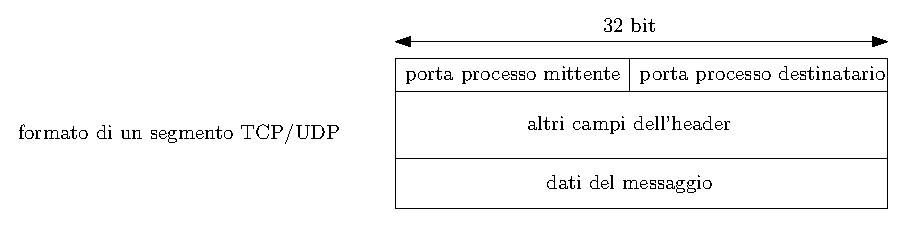
\includegraphics[width=0.9\textwidth ]{images/segmento.eps}
\end{center}
\subsubsection{Demultiplexing UDP e TCP}
Vediamo adesso come funziona il demultiplexing per i due differenti protocolli di trasporto, partendo con
UDP.\acc
Quando si crea un socket (canale virtuale), si deve specificare la porta locale del proprio host:\acc
\code{DatagramSocket mySocket1 = new DatagramSocket(12534);}
\acc
Per inviare un datagramma al socket UDP, bisogna specificare l'indirizzo IP di destinazione, e la porta del
processo di destinazione. Tramite l'IP, verrà individuato sulla rete l'host di destinazione, esso riceverà un
segmento UDP, verrà letto nell'header il campo relativo alla porta di destinazione, ed indirizzerà il
segmento al socket relativo a quel numero di porta.\acc
Per eseguire il demultiplexing nel destinatario, verrà utilizzato esclusivamente il numero di porta
del processo destinatario, il trasferimento UDP ha lo scopo di inviare un messaggio, e non di stabilire una
connessione, se arrivano ad un host due differenti datagrammi IP/UDP con la stessa porta di destinazione ma
diversi IP di origine (due diversi mittenti comunicano con lo stesso processo destinatario), semplicemente
entrambi i messaggi verranno indirizzati allo stesso socket ricevente.\acc
Nel caso del TCP, è differente, tale protocollo ha lo scopo di aprire una connessione persistente fra due
processi, ogni processo destinatario, non avrà un singolo socket che riceve tutti i segmenti, ma avrà
un socket per ogni connessione, quindi per ogni mittente.\acc
Un segmento IP/TCP quindi avrà bisogno di essere indirizzato nel socket corretto, non sarà più necessario
il numero di porta e l'IP del destinatario, ma per eseguire il demultiplexing, sarà anche necessario
distinguere i differenti host mittenti. \acc
Ogni socket sarà quindi identificato da una tupla composta da 4 valori:\begin{itemize}
    \item IP di origine
    \item Numero di porta di origine
    \item IP di destinazione
    \item Numero di porta di destinazione
\end{itemize}
Il multiplexing/demultiplexing non avviene però esclusivamente al livello di trasporto, ma anche su altri
livelli (verrà visto in seguito).
\subsection{UDP}
UDP è l'acronimo di \textit{User Datagram Protocol}, perché viene utilizzato il termine datagramma se si
parla di un segmento al livello di trasporto? Tale protocollo fornisce il servizio di trasporto senza
stabilire una connessione, è un sistema best-effort privo del concetto di handshake, si usa la parola datagramma
perché il segmento UDP è molto semplice, non c'è molta aggiunta di informazioni, l'header è molto piccolo.
\acc
Non c'è alcun controllo della congestione, un segmento UDP verrà inviato a prescindere dal traffico sulla
rete, viene utilizzato sulle applicazioni multimediali (streaming), dal DNS e da HTTP/3, che
gestisce il trasferimento affidabile a livello applicativo. \acc
Tale protocollo è estremamente semplice, non fa altro che ricevere un messaggio dall'applicazione, aggiungere
un header UDP, ed inviarlo al livello di rete, un segmento UDP ha il seguente formato:\begin{center}
    \includegraphics[width=0.9\textwidth ]{images/segmentoUDP.eps}
\end{center}
Il campo \textbf{checksum}, è un valore intero che serve a rilevare eventuali errori nel messaggio, quali
la modifica di alcuni bit dovuta ad interferenze elettromagnetiche. Quando viene composto un
segmento UDP, esso viene suddiviso in pezzi da 16 bit, che verranno trattati come un numero
intero in complemento ad 1, per poi essere sommati, dando quindi un valore che sarà appunto
il checksum.\acc
Il destinatario, si occuperà di eseguire lo stesso procedimento, ottenendo una somma, se essa differisce
dal campo checksum, vuol dire che c'è stato un errore ed alcuni bit sono cambiati, sarà poi compito
del destinatario decidere se scartare il segmento. Il checksum si imposta a zero nel caso non
si voglia utilizzare, esso è utilizzato su più livelli e non solo nei segmenti al livello di trasporto.
\subsection{Principi di Trasferimento Affidabile}
I protocolli al livello di trasporto non si occupano solo di creare
una comunicazione virtuale fra due processi su host diversi, ma anche di
garantire una comunicazione affidabile. Abbiamo visto come uno dei due
principali protocolli, l'UDP, non garantisce nulla di tutto ciò, in questo
capitolo si presenteranno dei concetti fondamentali, che saranno poi ripresi
dal TCP.\acc
Supponiamo di voler comunicare attraverso un canale in maniera
monodirezionale, ossia inviando dati esclusivamente da un host
all'altro. Per una comunicazione di questo tipo, è comunque necessario
un canale \textit{bidirezionale}, dato che l'host ricevente,
deve poter notificare al mittente di aver ricevuto correttamente il
messaggio.\acc
Ci occuperemo quindi di costruire un protocollo su un canale bidirezionale
\textit{inaffidabile}, la complessità del lavoro che dovrà impiegare tale
protocollo dipenderà dall'inaffibadilità del canale. Un altro problema
dipende dal fatto che il mittente ed il destinatario non conoscono
lo stato l'uno dell'altro.\acc
Costruiremo un astrazione di un protocollo chiamato
\textbf{rdt}, i dati viaggiano su un singolo canale, le informazioni di
controllo su entrambi i canali. Per descrivere il funzionamento del protocollo
useremo le \textbf{FSM}, ossia le macchine a stati finiti.
\subsubsection{rdt 1.0}
Costruiamo un'astrazione di un protocollo partendo da alcune assunzioni riguardanti possibili
inaffidabilità della comunicazione, aggiungendone sempre di più,
avvicinandoci ad un caso reale. Il protocollo rdt 1.0 si baserà su un
canale di comunicazione affidabile, in cui non ci sono perdite di
pacchetti o errori sui bit.\acc
Semplicemente, il mittente che riceve un messaggio dal livello applicativo,
lo incapsulerà in un pacchetto, per poi inviarlo ai livelli inferiori.
Il destinatario riceverà il pacchetto dai livelli inferiori,
effettuerà il decapsulamento ed invierà il messaggio al giusto
processo tramite il numero di porta.\begin{center}
    \includegraphics[width=\textwidth ]{images/rdt1.0.eps}
\end{center}
Risulta molto semplice tale implementazione data l'assunzione di un
canale totalmente affidabile.\acc
\textbf{Appunto sulla notazione} : \begin{itemize}
    \item rdt\_send(data) - il protocollo invia il messaggio al
          destinatario.
    \item packet = make\_packet(data) - il messaggio da inviare viene
          incapsulato in un pacchetto.
    \item udt\_send(data) - il pacchetto incapsulato viene inviato
          al socket tramite un protocollo inaffidabile.
    \item rdt\_receive(packet) - il protocollo riceve il pacchetto dal mittente. 
    \item extract(packet,data) - il protocollo si occupa di eseguire il decapsulamento del pacchetto,
    data conterrà il messaggio estratto. 
    \item deliver\_data(data) - il messaggio estratto viene inviato all'applicazione.
\end{itemize}
\subsubsection{rdt 2.0}
Consideriamo adesso un canale che non è al 100\% affidabile, ossia che, con una certa probabilità, 
causi degli \textit{errori} sui bit, che dovranno essere rilevati tramite il campo checksum\footnote{
    si assume che il checksum sia infallibile e rilevi sempre errori, se presenti
} nell'header.
Sono necessari i seguenti costrutti: 
\begin{itemize}
    \item Con il termine \textbf{ACK}, si intende un pacchetto che il destinatario invia al mittente in seguito 
    alla ricezione di un messaggio, ed ha lo 
    scopo di notificare a quest'ultimo che tale messaggio non presenta errori nei bit.
    \item Con il termine \textbf{NAK}, si intende un pacchetto che il destinatario invia al mittente in seguito 
    alla ricezione di un messaggio, ed ha lo 
    scopo di notificare a quest'ultimo che tale messaggio presenta errori nei bit, appositamente rilevati 
    tramite il checksum.
\end{itemize}
Se il destinatario dovesse notificare un NAK, sarà necessario re-inviare il pacchetto che è stato modificato. 
Per ragioni di semplicità, tale protocollo utilizzerà una politica di invio pacchetti \textbf{stop-and-wait}, 
consiste nell'inviare un singolo pacchetto alla volta, ed inviare il pacchetto successivo solo quando 
si ha la certezza che quello precedente sia stato consegnato.\begin{center}
    \includegraphics[width=1\textwidth ]{images/rdt2.0.eps}
\end{center}
Il protocollo è ancora relativamente semplice, il mittente dopo aver inviato il pacchetto, attende di ricevere un 
ACK oppure un NAK, nel primo caso, passerà al prossimo pacchetto, altrimenti, si occuperà di re-inviare il pacchetto 
corrotto. Il destinatario invece, si occuperà semplicemente di ricevere pacchetti, controllare se sono corrotti tramite 
l'operazione \code{is\_corrupt(packet)}, ed inviare un eventuale ACK o NAK al destinatario. 
C'è però un assunzione in questo modello che non è stata considerata.
\subsubsection{rdt 2.1} 
L'rdt 2.1 si occupa di gestire anche un possibile errore sui bit dei pacchetti ACK/NAK, un pacchetto corrotto di questo 
tipo non può essere interpretato dal mittente, quindi come soluzione, quest'ultimo ri-invierà il pacchetto, se il messaggio 
corrotto però in origine era un ACK, si avrà un pacchetto duplicato che il destinatario dovrà scartare.\acc 
Ad ogni pacchetto verrà aggiunto un numero di controllo, che identificherà il numero di sequenza del pacchetto, al 
destinatario sarà necessario leggerlo per controllare se tale pacchetto è nuovo oppure è una ritrasmissione 
del pacchetto precedente, scaturita da un ACK/NAK corrotto. Tale numero di sequenza sarà implementato con un singolo 
bit, che può essere 0 oppure 1, nel modello stop-and-wait sono necessari solo questi due valori.\begin{center}
    \includegraphics[width=0.9\textwidth ]{images/rdt2.1.eps}
\end{center} 
Il mittente manda il pacchetto 0, se riceve un ACK/NAK corrotto, lo ri-invierà, se il destinatario si aspettava un pacchetto 
1, in quanto aveva ricevuto correttamente il pacchetto 0, scarterà il pacchetto.
\subsubsection{rdt 3.0}
Il problema principale che non è ancora stato considerato riguarda l'eventualità che un pacchetto venga 
\textit{perso}, ebbene è un evento molto comune nelle reti, e se si vuole garantire un trasferimento affidabile, 
si deve considerare un modo per evitare tale perdita, mantenendo l'integrità dei dati.\acc 
Supponiamo nell'rdt 3.0, che il canale possa causare una perdita di pacchetto, il mittente dovrà accertarsi che ogni pacchetto 
inviato sia ricevuto, il destinatario non è al corrente dello stato del mittente, quindi esso potrebbe essere totalmente 
ignaro che un pacchetto a lui destinato è stato perso.\acc 
Il mittente, sa che un pacchetto è stato perso se non riceverà alcun ACK (o NAK) da parte del destinatario, per ogni pacchetto 
inviato sarà quindi previsto un \textit{timer}, se entro un lasso di tempo stabilito, il mittente non riceverà alcun messaggio 
di ACK, il pacchetto sarà considerato perso, e sarà inviato nuovamente.\begin{center}
    \includegraphics[width=1\textwidth ]{images/rdt3.0.eps}
\end{center} 
Se viene ricevuto un pacchetto ACK con un numero non atteso, non viene fatto nulla, in quanto scatterà ugualmente 
il timeout, non vengono più usati pacchetti ACK e NAK, ma esclusivamente pacchetti ACK. 
\subsubsection{Pipelining}
Il problema è che tale protocollo convive con le restrizioni di un paradigma stop-and-wait, e l'attesa di un round trip 
time per ogni pacchetto prima di poter inviare il prossimo riduce drasticamente le prestazioni, bisogna utilizzare un modello 
di \textit{pipelining}, ossia includere la possibilità per il mittente, che esso possa inviare pacchetti senza dover 
attendere che quelli precedenti siano stati correttamente consegnati. Vediamo i due paradigmi di pipelining principali.\acc 
Il modello \textbf{go-back-n} permette al mittente di trasmettere più pacchetti contemporaneamente, può inviare al destinatario 
al più $n$ pacchetti senza riceverne i rispettivi ACK. Alla ricezione di ogni pacchetto, il destinatario invierà un 
ACK \textbf{comulativo}, i pacchetti sono numerati ed ordinati in sequenza, ed un ACK di numero $x$ indica che sono 
stati ricevuti tutti i pacchetti sino al pacchetto $x$, e se ne necessitano dall'$x+1$-esimo in poi.\acc 
Il timer, farà riferimento al pacchetto più "vecchio" inviato del quale non è stato ricevuto l'ACK, se scade, 
verranno re-inviati tutti gli $n$ pacchetti da quest'ultimo in poi. I pacchetti che sono stati ricevuti ma in un ordine 
sbagliato (ad esempio, si è in attesa del pacchetto 3 ma viene consegnato il pacchetto 4) verranno scartati, oppure 
memorizzati in un buffer.\begin{center}
    \includegraphics[width=1\textwidth ]{images/go-back-n.eps}
\end{center} 
L'altro costrutto di pipelining è noto con il nome di \textbf{selective repeat}, piuttosto che inviare un ACK 
comulativo, ne viene inviato uno \textbf{selettivo}, riservato ad ogni singolo pacchetto, i pacchetti arrivati
in un ordine sbagliato, verranno salvati in un buffer, in questo modo, il mittente avrà una finestra di $n$ pacchetti 
da poter inviare, ed il destinatario avrà una finestra di $n$ pacchetti da poter mantenere nel buffer, inoltre ogni 
pacchetto ha il suo personale timer.\acc 
Tale metodo risulta efficiente in quanto non è necessario dover inviare nuovamente l'intera finestra di $n$ pacchetti, 
e riduce il grado di ridondanza, inoltre se la rete è congestionata, la rispedizione di tutti i pacchetti 
peggiora la congestione. \acc 
Il destinatario salverà i pacchetti nel buffer, quando avrà a disposizione la giusta sequenza ordinata, li invierà 
al livello applicativo, decapsulandoli.\begin{center}
    \includegraphics[width=1\textwidth ]{images/selectiveRepeat.eps}
\end{center} 
Anche se tale astrazione è stata costruita per una comunicazione mono-direzionale, nulla vita ad un pacchetto che 
trasporta i dati, di trasportare anche i riscontri ACK, tale tecnica è nota con il nome di \textit{piggy-backing}, 
permettendo a due enti di comunicare e contemporaneamente notificarsi dell'ascolto.\acc 
Un problema noto del selective repeat risiede nelle dimensioni della finestra del ricevitore, la mancata sincronizzazione 
fra la finestra del mittente e quest'ultima causa gravi conseguenze quando si ha a che fare con un intervallo finito 
di numeri di sequenza, si osservi il seguente esempio, in cui il range di numeri di sequenza per i 
pacchetti sono [0,1,2,3] e la finestra del ricevitore ha ampiezza 3:\begin{center}
    \includegraphics[width=\textwidth ]{images/ErroreSelectiveRepeat.eps}
\end{center} 
Il primo pacchetto ed il quinto pacchetto, hanno entrambi numero di sequenza 0. Il mittente, riceve correttamente
i primi tre pacchetti, con numeri di sequenza 0, 1 e 2, e la sua finestra verrà spostata sui pacchetti 
3, 0 ed 1, che sono rispettivamente il quarto, il quinto ed il sesto.\acc 
Il fatto è che, a seguito della perdita dei pacchetti ACK, il mittente non sa che i primi tre pacchetti sono stati 
ricevuti, ri-invierà quindi il primo pacchetto con numero di sequenza 0 a seguito del timeout. Qui, il destinatario, 
sta attendendo il quinto pacchetto che ha numero di sequenza 0, e riceve il primo pacchetto, anche esso con numero di 
sequenza 0.\acc 
Il destinatario interpreterà il primo pacchetto come se fosse il quinto, essendo che essi hanno lo stesso numero di 
sequenza, tale errore causa una grave corruzione dei dati ricevuti.\acc 
Per evitare ciò, è necessario sincronizzare l'ampiezza della finestra del destinatario, con la sequenza dei 
numeri dei pacchetti, secondo tale relazione: \begin{itemize}
    \item Se i numeri di sequenza sono $2^m$ (Ad esempio, [0,1,2,3] sono $2^2$).
    \item La finestra del ricevitore deve essere grande $2^{m-1}$ (Ad esempio : $2^{2-1}=2^1=2$).
\end{itemize}
\subsection{TCP - parte 1 : Affidabilità e Connessione}
\subsubsection{Struttura del Segmento}
Il protocollo TCP vede il trasferimento dei dati, non come l'invio di segmenti, ma come l'invio di un 
flusso di byte che compongono i messaggi, tale flusso deve arrivare dal mittente al destinatario in un 
preciso ordine, è un protocollo bidirezionale che prevede una misura massima per la dimensione dei segmenti, 
detta $MSS$ (solitamente 1460 byte).\acc 
Il TCP permette ai due enti che comunicano di stabilire una connessione virtuale, di cui il resto della rete 
non è a conoscenza. Utilizza dei riscontri ACK comulativi, e sfrutta il pipelining per l'invio di più 
pacchetti. Con il termine \textbf{handshake}, si intende l'azione in cui i due enti stabiliscono la 
connessione, tramite dei messaggi di controllo. Un segmento TCP è lo stesso sia per un messaggio di invio dati, sia 
che per un messaggio di ACK (dato che utilizza il piggy-backing), ed è il seguente:\begin{center}
    \includegraphics[width=0.5\textwidth ]{images/TCPsegment.eps}
\end{center} 
Il numero di sequenza non si riferisce al numero d'ordine del segmento, ma si riferisce al numero d'ordine 
del primo byte del segmento di cui fa riferimento.\begin{quote}\color{gray}
    Ad esempio, si vuole mandare un messaggio di 10 byte, verrà incapsulato in 2 segmenti TCP di 
    5 byte ciascuno, il primo segmento conterrà i byte dal numero 1 al numero 5, avrà quindi numero di 
    sequenza 1, il secondo segmento conterrà i byte dal numero 6 al numero 10, avrà quindi numero di 
    sequenza 6.\color{black}
\end{quote}
Il numero dell'ACK fa riferimento al byte successivo atteso, un numero di ACK $x$ indica che sono stati ricevuti tutti 
i byte dal primo fino al $x-1$ esimo (l'ACK è comulativo). Il campo \textit{"INFO"} contiene delle informazioni come il numero di lunghezza 
dell'header, un flag che indica se il checksum è in utilizzo oppure no, dei flag riguardo la gestione/sincronizzazione 
della connessione ed altre informazioni.\acc 
Il campo \textit{"finestra del ricevitore"} indica il numero di byte che il destinatario può "accogliere", 
 è necessario per il controllo del flusso, se il destinatario è "ingolfato", tale numero 
di byte sarà più basso, imponendo al mittente di porre limite al numero di pacchetti che può inviare, per non intasare 
ulteriormente la connessione. Il campo \textit{"opzioni aggiuntive"} contiene informazioni come la lunghezza 
del messaggio.\acc 
La gestione dei segmenti arrivati fuori ordine, non è considerata dal TCP, bensì dipende dall'implementazione.
\subsubsection{Gestione del Timer}
Abbiamo visto che un protocollo che ha lo scopo di garantire un trasferimento affidabile deve servirsi di un timeout 
per la ritrasmissione dei pacchetti andati perduti, ma come va dosato il tempo effettivo di durata del timer?\acc 
È chiaro che, il timeout deve essere almeno uguale o superiore al RTT (\textit{round trip time}), altrimenti ogni pacchetto 
inviato scadrebbe in un timeout, il punto è che il RTT è variabile, e deve essere misurato da un timer, chiameremo 
il tempo di RTT effettivo misurato dal timer $sampleRTT$, tramite tale misurazione per un pacchetto,
 vogliamo stimare il RTT del pacchetto successivo, mantenendo la stima regolare, senza che sia troppo condizionata dalle 
 oscillazioni (variabilità) del $sampleRTT$.\acc 
 Viene utilizzata una tecnica nota come \textbf{EWMA} (exponential waited moving avarage), che tramite l'uso di un 
 peso $\alpha$ (numero reale fra 0 ed 1), utilizza le misurazioni precedenti per stimare il RTT successivo. Si indica con 
 $RTTstimato(t)$, la stima del RTT al tempo $t$, si ha che:
 $$ RTTstimato(t) = (1-\alpha)\cdot RTTstimato(t-1)+\alpha \cdot SampleRTT$$
 Se $\alpha = \nicefrac{1}{2}$, il RTT stimato sarà una media fra il RTT precedentemente stimato e quello 
 precedentemente misurato. Un valore tipico che si utilizza è $\alpha=0.125$.\acc 
 Il time out necessita inoltre di un minimo spazio, margine di sicurezza, in modo da essere di poco superiore 
 al RTT stimato, il valore effettivo che verrà utilizzato per il timeout, sarà pesato da tale margine di sicurezza 
 noto come $DevRTT$, misura la precisione della stima, ed è influenzato dalla variabilità del $SampleRTT$.
 $$ DevRTT(t) = (1-\beta)\cdot DevRTT(t-1) + \beta\cdot(|SampleRTT-RTTstimato(t-1)|) $$
 Dove $\beta$ è un numero reale fra 0 ed 1, viene utilizzato come peso, il valore 
 $|SampleRTT-RTTstimato(t-1)|$ non è altro che la differenza fra il RTT stimato ed il 
 RTT effettivo. Il tempo effettivo del timeout sarà:
 $$ timeout=RTTstimato+4\cdot DevRTT$$
 Si osservi il seguente grafico che mostra la differenza fra il RTT misurato ed il RTT stimato (quest'ultimo risulta 
 regolare e meno soggetto ad oscillazioni).\begin{center}
    \includegraphics[width=\textwidth ]{images/RTTstimato.eps}
\end{center} 
\subsubsection{Semplificazione del TCP, Gestione del Flusso e della Connessione}
Vediamo adesso il funzionamento del TCP in maniera approssimativa, cominciando dal ruolo del \textbf{mittente}, 
esso riceve un messaggio dal livello applicativo, tale messaggio viene incapsulato in un segmento TCP con 
l'aggiunta di un header, dopo di che, se non vi è già un timer in esecuzione, viene avviato (si ricordi che 
è in esecuzione un solo timer valido per il segmento inviato meno recentemente per la quale non si è ricevuto 
ancora l'ACK).\acc 
All'avvenimento di un timeout, il mittente dovrà ri-inviare il segmento in questione, riavviando anche il timer. 
Alla ricezione di un ACK (che si ricorda essere comulativo), viene aggiornata la finestra di pacchetti 
da inviare, se vi sono ancora pacchetti il cui invio non è confermato, partirà un timer associato al pacchetto 
inviato meno recentemente fra questi ultimi.\acc Vediamo il comportamento del \textbf{destinatario}:\begin{itemize}
    \item \textbf{evento} : arrivo di un segmento in ordine,
    con numero di segmento atteso, 
   ossia per cui tutti i segmenti precedenti  ad esso sono 
   già stati confermati  (situazione regolare) \\ \textbf{risposta} : si attende un tempo (solitamente 500ms) prima 
   di inviare l'ACK, questo delay serve a coprire 
   situazioni in cui, dovesse arrivare un nuovo segmento (successivo a
    quello originale)  pochi istanti dopo (riducendo il numero di ACK
    complessivi inviati).
    \item \textbf{evento} :arrivo di un segmento in ordine, con numero
    di segmento atteso,  ma un segmento precedente ricevuto,
    non è ancora stato confermato 
   tramite l'invio di un ACK (complementare
    all'evento precedente)\\
    \textbf{risposta} : si invia immediatamente un ACK comulativo,
    confermando entrambi i segmenti.
    \item \textbf{evento} : arrivo di un segmento fuori ordine\\
    \textbf{risposta} : si invia immediatamente un ACK duplicato in
    cui si richiede il segmento atteso in ordine
    \item \textbf{evento} : arrivo di un segmento che riempie
    parzialmente o completamente un gap\\
    \textbf{risposta} : si invia immediatamente un ACK 
\end{itemize}
Nell'ultimo caso, in cui si parla di "gap" da riempire, si intende una situazione in cui il destinatario ha confermato 
(ad esempio), i segmenti 1,2 e 3, è in attesa del 4, ma mantiene nel buffer i segmenti 5 e 6, l'arrivo del 
segmento 4, farà si che verranno mandati al livello applicativo i segmenti 4,5 e 6, facendo si che il destinatario 
invia un ACK comulativo con numero 7 (si ricordi che il numero di segmento si riferisce ai byte e non al segmento 
stesso, sono stati utilizzati numeri sequenziali per semplicità, nell'assunzione che ogni segmento abbia 1 byte).\acc 
Si osservi la seguente situazione:\begin{center}
    \includegraphics[width=\textwidth ]{images/fastRetrasmit.eps}
\end{center} 
Introduciamo il \textbf{controllo del flusso}, si consideri uno scenario, dalla parte di un destinatario 
TCP, in cui il livello di rete fornisce segmenti più rapidamente rispetto a quanto il livello di applicazione 
possa leggerne, riempendo il buffer del socket TCP. \acc In tal caso il destinatario, dovrà notificare il mittente del 
fatto che esso sta trasmettendo troppo \textit{rapidamente}, almeno più di quanto esso possa processare i 
segmenti. Il destinatario avviserà il mittente tramite gli appositi campi nell'header relativi alla sua finestra 
di ricezione.\acc 
Si osservi come questa è una congestione \textit{locale}, e non da parte della rete, può avvenire anche se la rete 
è totalmente libera, e dipende eslcusivamente dalla velocità di elaborazione dei segmenti del destinatario.\acc 
Il destinatario TCP "dichiara" lo spazio che ha libero per i segmenti nel buffer tramite il 
campo \code{rwnd} nell'header, ed il mittente imposta la sua finestra di segmenti possibilmente 
inviabili prima di essere confermati, proprio al valore di \code{rwnd}, ciò garantisce l'assenza di 
sovraccaricamento nel buffer del ricevitore.\acc 
Il TCP si occupa anche di creare una \textbf{connessione} stabile fra i due comunicatori, tramite la già 
citata operazione di \textbf{handshake} (stretta di mano). Consiste, nella dichiarazione da parte dei due comunicatori 
di voler aprire una connessione (richiesta ed accettazione), e nel concordamento di alcuni parametri, quali il 
numero di porta, la finestra di ricezione, oppure il numero iniziale di segmento atteso.\acc 
Inizialmente il TCP si serviva di un handshake \textit{a 2 vie}:\begin{enumerate}
    \item 
 colui che voleva aprire la connessione (richiedente) 
inviava una richiesta di connessione ad un host (richiesto), tale richiesta era accompagnata da un numero 
$x$.     \item  il richiesto, rispondeva con un messaggio di "accettazione", re-inviando il numero $x$ per indicare 
che la risposta è relativa alla richiesta dello stesso numero.
\item a quel punto, il richiedente era pronto ad inviare dati, inviando però, anche un valore numerico aggiuntivo, 
ossia $x+1$. 
\item il richiesto, riceve i dati, ed invia un messaggio di ACK, con numero di sequenza $x+1$, alla ricezione di quest'ultimo 
la connessione sarà ufficialmente stabilita.
\end{enumerate}
In alcuni scenari, l'handshake a 2 vie può risultare problematico, ad esempio quando il richiedente si disconnette 
durante una richiesta di connessione, lasciando una connessione "aperta", per questo le implementazioni odierne del TCP 
implementano l'handshake \textit{a 3 vie}:\begin{enumerate}
    \item il richiedente, sceglie un numero $x$, ed invia un messaggio TCP SYN. 
    \item il richiesto che riceve il messaggio, sceglie un numero $y$, che sarà il primo numero di 
    sequenza, ed invia al richiedente un ACK, con numero di sequenza richiesto $y$, insieme ad un valore aggiuntivo,
    ossia $x+1$. 
    \item il richiedente riceverà il messaggio, verificando di aver ricevuto $x+1$, ciò indicherà che il 
    richiesto è attivo, invierà poi un segmento (possibilmente 
    già provvisto di dati), con numero di ACK $y+1$. 
    \item il richiesto, una volta ricevuto il segmento con ACK $y+1$, avrà la certezza che il richiedente è attivo, 
    e la connessione sarà ufficialmente stabilita.
\end{enumerate}
Tali numeri $x$ ed $y$ stabiliscono quindi il numero di sequenza iniziale, che molto spesso non è 0, infatti, 
per ragioni di sicurezza,  tali due numeri sono selezionati casualmente.\acc
Quando una connessione deve essere \textit{chiusa}, colui che ha intenzione di interromperla invierà un segmento 
con un flag \code{FIN=1}, colui che lo riceverà, risponderà con un ACK combinato con il proprio \code{FIN}, 
confermando la chiusura della connessione.
\subsection{TCP - parte 2 : Controllo della Congestione }
\end{document}
